% **************************************************************************************************************
% A Classic Thesis Style
% An Homage to The Elements of Typographic Style
%
% Copyright (C) 2011 Andr\'e Miede http://www.miede.de
%
% If you like the style then I would appreciate a postcard. My address 
% can be found in the file ClassicThesis.pdf. A collection of the 
% postcards I received so far is available online at 
% http://postcards.miede.de
%
% License:
% This program is free software; you can redistribute it and/or modify
% it under the terms of the GNU General Public License as published by
% the Free Software Foundation; either version 2 of the License, or
% (at your option) any later version.
%
% This program is distributed in the hope that it will be useful,
% but WITHOUT ANY WARRANTY; without even the implied warranty of
% MERCHANTABILITY or FITNESS FOR A PARTICULAR PURPOSE.  See the
% GNU General Public License for more details.
%
% You should have received a copy of the GNU General Public License
% along with this program; see the file COPYING.  If not, write to
% the Free Software Foundation, Inc., 59 Temple Place - Suite 330,
% Boston, MA 02111-1307, USA.
%
% **************************************************************************************************************
% Note:
%    * You must not use "u etc. in strings/commands that will be spaced out (use \"u or real umlauts instead)
%    * New enumeration (small caps): \begin{aenumerate} \end{aenumerate}
%    * For margin notes: \marginpar or \graffito{}
%    * Do not use bold fonts in this style, it is designed around them
%    * Use tables as in the examples
%    * See classicthesis-preamble.sty for useful commands
% **************************************************************************************************************
% To Do:
%		 * [high] Check this out: http://www.golatex.de/koma-script-warnung-in-verbindung-mit-listings-package-t2058.html
%    * [medium] mathbb in section-titles/chapter-titles => disappears somehow in headlines!!!
% **************************************************************************************************************
\documentclass[ twoside,openright,titlepage,numbers=noenddot,headinclude,%1headlines,% letterpaper a4paper
                footinclude=true,cleardoublepage=empty,abstractoff, % <--- obsolete, remove (todo)
                BCOR=5mm,paper=a4,fontsize=11pt,%11pt,a4paper,%
                ]{scrbook}

%********************************************************************
% Note: Make all your adjustments in here
%*******************************************************
% ****************************************************************************************************
% classicthesis-config.tex 
% formerly known as loadpackages.sty, classicthesis-ldpkg.sty, and classicthesis-preamble.sty 
% Use it at the beginning of your ClassicThesis.tex, or as a LaTeX Preamble 
% in your ClassicThesis.{tex,lyx} with % ****************************************************************************************************
% classicthesis-config.tex 
% formerly known as loadpackages.sty, classicthesis-ldpkg.sty, and classicthesis-preamble.sty 
% Use it at the beginning of your ClassicThesis.tex, or as a LaTeX Preamble 
% in your ClassicThesis.{tex,lyx} with % ****************************************************************************************************
% classicthesis-config.tex 
% formerly known as loadpackages.sty, classicthesis-ldpkg.sty, and classicthesis-preamble.sty 
% Use it at the beginning of your ClassicThesis.tex, or as a LaTeX Preamble 
% in your ClassicThesis.{tex,lyx} with \input{classicthesis-config}
% ****************************************************************************************************  
% If you like the classicthesis, then I would appreciate a postcard. 
% My address can be found in the file ClassicThesis.pdf. A collection 
% of the postcards I received so far is available online at 
% http://postcards.miede.de
% ****************************************************************************************************


%my packages

\usepackage[tight]{units}
\usepackage{nicefrac}
\usepackage{macros}
% ****************************************************************************************************
% 1. Configure classicthesis for your needs here, e.g., remove "drafting" below 
% in order to deactivate the time-stamp on the pages
% ****************************************************************************************************
\PassOptionsToPackage{eulerchapternumbers,listings,drafting,%
				 pdfspacing,%floatperchapter,%linedheaders,%
				 subfig,beramono,eulermath,parts}{classicthesis}										
% ********************************************************************
% Available options for classicthesis.sty 
% (see ClassicThesis.pdf for more information):
% drafting
% parts nochapters linedheaders
% eulerchapternumbers beramono eulermath pdfspacing minionprospacing
% tocaligned dottedtoc manychapters
% listings floatperchapter subfig
% ********************************************************************

% ********************************************************************
% Triggers for this config
% ******************************************************************** 
\usepackage{ifthen}
\newboolean{enable-backrefs} % enable backrefs in the bibliography
\setboolean{enable-backrefs}{false} % true false
% ****************************************************************************************************


% ****************************************************************************************************
% 2. Personal data and user ad-hoc commands
% ****************************************************************************************************
\newcommand{\myTitle}{A search for exotic particles of charge
    \nicefrac{5}{3} with the CMS detector\xspace}
\newcommand{\mySubtitle}{\xspace}
\newcommand{\myDegree}{\xspace}
\newcommand{\myName}{Matteo Abis\xspace}
\newcommand{\myProf}{Patrizia Azzi\xspace}
\newcommand{\myOtherProf}{\xspace}
\newcommand{\mySupervisor}{\xspace}
\newcommand{\myFaculty}{\xspace}
\newcommand{\myDepartment}{Dipartimento di Fisica e Astronomia\xspace}
\newcommand{\myUni}{Universit\`a degli Studi di Padova\xspace}
\newcommand{\myLocation}{\xspace}
\newcommand{\myTime}{A.A. 2011/2012\xspace}
\newcommand{\myVersion}{\xspace}

% ********************************************************************
% Setup, finetuning, and useful commands
% ********************************************************************
\newcounter{dummy} % necessary for correct hyperlinks (to index, bib, etc.)
\newlength{\abcd} % for ab..z string length calculation
\providecommand{\mLyX}{L\kern-.1667em\lower.25em\hbox{Y}\kern-.125emX\@}
\newcommand{\ie}{i.\,e.}
\newcommand{\Ie}{I.\,e.}
\newcommand{\eg}{e.\,g.}
\newcommand{\Eg}{E.\,g.} 
% ****************************************************************************************************


% ****************************************************************************************************
% 3. Loading some handy packages
% ****************************************************************************************************
% ******************************************************************** 
% Packages with options that might require adjustments
% ******************************************************************** 
\PassOptionsToPackage{utf8x}{inputenc}	% latin9 (ISO-8859-9) = latin1+"Euro sign"
 \usepackage{inputenc}				

%\PassOptionsToPackage{ngerman,american}{babel}   % change this to your language(s)
% Spanish languages need extra options in order to work with this template
%\PassOptionsToPackage{spanish,es-lcroman}{babel}
 \usepackage[italian,UKenglish]{babel}					

\PassOptionsToPackage{square,numbers}{natbib}
 \usepackage{natbib}				

\PassOptionsToPackage{fleqn}{amsmath}		% math environments and more by the AMS 
 \usepackage{amsmath}

% ******************************************************************** 
% General useful packages
% ******************************************************************** 
\PassOptionsToPackage{T1}{fontenc} % T2A for cyrillics
	\usepackage{fontenc}                 
\usepackage{xspace} % to get the spacing after macros right  
\usepackage{mparhack} % get marginpar right
\usepackage{fixltx2e} % fixes some LaTeX stuff 
\PassOptionsToPackage{printonlyused,smaller}{acronym}
	\usepackage{acronym} % nice macros for handling all acronyms in the thesis
%\renewcommand*{\acsfont}[1]{\textssc{#1}} % for MinionPro
\renewcommand{\bflabel}[1]{{#1}\hfill} % fix the list of acronyms
% ****************************************************************************************************


% ****************************************************************************************************
% 4. Setup floats: tables, (sub)figures, and captions
% ****************************************************************************************************
\usepackage{tabularx} % better tables
	\setlength{\extrarowheight}{3pt} % increase table row height
\newcommand{\tableheadline}[1]{\multicolumn{1}{c}{\spacedlowsmallcaps{#1}}}
\newcommand{\myfloatalign}{\centering} % to be used with each float for alignment
\usepackage{caption}
\captionsetup{format=hang,font=small}
\usepackage{subfig}  
% ****************************************************************************************************


% ****************************************************************************************************
% 5. Setup code listings
% ****************************************************************************************************
\usepackage{listings} 
%\lstset{emph={trueIndex,root},emphstyle=\color{BlueViolet}}%\underbar} % for special keywords
\lstset{language=[LaTeX]Tex,%C++,
    keywordstyle=\color{RoyalBlue},%\bfseries,
    basicstyle=\small\ttfamily,
    %identifierstyle=\color{NavyBlue},
    commentstyle=\color{Green}\ttfamily,
    stringstyle=\rmfamily,
    numbers=none,%left,%
    numberstyle=\scriptsize,%\tiny
    stepnumber=5,
    numbersep=8pt,
    showstringspaces=false,
    breaklines=true,
    frameround=ftff,
    frame=single,
    belowcaptionskip=.75\baselineskip
    %frame=L
} 
% ****************************************************************************************************    		   


% ****************************************************************************************************
% 6. PDFLaTeX, hyperreferences and citation backreferences
% ****************************************************************************************************
% ********************************************************************
% Using PDFLaTeX
% ********************************************************************
\PassOptionsToPackage{pdftex,hyperfootnotes=false,pdfpagelabels}{hyperref}
	\usepackage{hyperref}  % backref linktocpage pagebackref
\pdfcompresslevel=9
\pdfadjustspacing=1 
\PassOptionsToPackage{pdftex}{graphicx}
	\usepackage{graphicx} 

% ********************************************************************
% Setup the style of the backrefs from the bibliography
% (translate the options to any language you use)
% ********************************************************************
\newcommand{\backrefnotcitedstring}{\relax}%(Not cited.)
\newcommand{\backrefcitedsinglestring}[1]{(Cited on page~#1.)}
\newcommand{\backrefcitedmultistring}[1]{(Cited on pages~#1.)}
\ifthenelse{\boolean{enable-backrefs}}%
{%
		\PassOptionsToPackage{hyperpageref}{backref}
		\usepackage{backref} % to be loaded after hyperref package 
		   \renewcommand{\backreftwosep}{ and~} % separate 2 pages
		   \renewcommand{\backreflastsep}{, and~} % separate last of longer list
		   \renewcommand*{\backref}[1]{}  % disable standard
		   \renewcommand*{\backrefalt}[4]{% detailed backref
		      \ifcase #1 %
		         \backrefnotcitedstring%
		      \or%
		         \backrefcitedsinglestring{#2}%
		      \else%
		         \backrefcitedmultistring{#2}%
		      \fi}%
}{\relax}    

% ********************************************************************
% Hyperreferences
% ********************************************************************
\hypersetup{%
    %draft,	% = no hyperlinking at all (useful in b/w printouts)
    colorlinks=true, linktocpage=true, pdfstartpage=3, pdfstartview=FitV,%
    % uncomment the following line if you want to have black links (e.g., for printing)
    %colorlinks=false, linktocpage=false, pdfborder={0 0 0}, pdfstartpage=3, pdfstartview=FitV,% 
    breaklinks=true, pdfpagemode=UseNone, pageanchor=true, pdfpagemode=UseOutlines,%
    plainpages=false, bookmarksnumbered, bookmarksopen=true, bookmarksopenlevel=1,%
    hypertexnames=true, pdfhighlight=/O,%nesting=true,%frenchlinks,%
    urlcolor=webbrown, linkcolor=RoyalBlue, citecolor=webgreen, %pagecolor=RoyalBlue,%
    %urlcolor=Black, linkcolor=Black, citecolor=Black, %pagecolor=Black,%
    pdftitle={\myTitle},%
    pdfauthor={\textcopyright\ \myName, \myUni, \myFaculty},%
    pdfsubject={},%
    pdfkeywords={},%
    pdfcreator={pdfLaTeX},%
    pdfproducer={LaTeX with hyperref and classicthesis}%
}   

% ********************************************************************
% Setup autoreferences
% ********************************************************************
% There are some issues regarding autorefnames
% http://www.ureader.de/msg/136221647.aspx
% http://www.tex.ac.uk/cgi-bin/texfaq2html?label=latexwords
% you have to redefine the makros for the 
% language you use, e.g., american, ngerman
% (as chosen when loading babel/AtBeginDocument)
% ********************************************************************
\makeatletter
\@ifpackageloaded{babel}%
    {%
       \addto\extrasamerican{%
					\renewcommand*{\figureautorefname}{Figure}%
					\renewcommand*{\tableautorefname}{Table}%
					\renewcommand*{\partautorefname}{Part}%
					\renewcommand*{\chapterautorefname}{Chapter}%
					\renewcommand*{\sectionautorefname}{Section}%
					\renewcommand*{\subsectionautorefname}{Section}%
					\renewcommand*{\subsubsectionautorefname}{Section}% 	
				}%
       \addto\extrasngerman{% 
					\renewcommand*{\paragraphautorefname}{Absatz}%
					\renewcommand*{\subparagraphautorefname}{Unterabsatz}%
					\renewcommand*{\footnoteautorefname}{Fu\"snote}%
					\renewcommand*{\FancyVerbLineautorefname}{Zeile}%
					\renewcommand*{\theoremautorefname}{Theorem}%
					\renewcommand*{\appendixautorefname}{Anhang}%
					\renewcommand*{\equationautorefname}{Gleichung}%        
					\renewcommand*{\itemautorefname}{Punkt}%
				}%	
			% Fix to getting autorefs for subfigures right (thanks to Belinda Vogt for changing the definition)
			\providecommand{\subfigureautorefname}{\figureautorefname}%  			
    }{\relax}
\makeatother


% ****************************************************************************************************
% 7. Last calls before the bar closes
% ****************************************************************************************************
% ********************************************************************
% Development Stuff
% ********************************************************************
\listfiles
%\PassOptionsToPackage{l2tabu,orthodox,abort}{nag}
%	\usepackage{nag}
%\PassOptionsToPackage{warning, all}{onlyamsmath}
%	\usepackage{onlyamsmath}

% ********************************************************************
% Last, but not least...
% ********************************************************************
\usepackage{classicthesis} 
% ****************************************************************************************************


% ****************************************************************************************************
% 8. Further adjustments (experimental)
% ****************************************************************************************************
% ********************************************************************
% Changing the text area
% ********************************************************************
%\linespread{1.05} % a bit more for Palatino
%\areaset[current]{312pt}{761pt} % 686 (factor 2.2) + 33 head + 42 head \the\footskip
%\setlength{\marginparwidth}{7em}%
%\setlength{\marginparsep}{2em}%

% ********************************************************************
% Using different fonts
% ********************************************************************
%\usepackage[oldstylenums]{kpfonts} % oldstyle notextcomp
%\usepackage[osf]{libertine}
%\usepackage{hfoldsty} % Computer Modern with osf
%\usepackage[light,condensed,math]{iwona}
%\renewcommand{\sfdefault}{iwona}
%\usepackage{lmodern} % <-- no osf support :-(
%\usepackage[urw-garamond]{mathdesign} <-- no osf support :-(
% ****************************************************************************************************

% ****************************************************************************************************  
% If you like the classicthesis, then I would appreciate a postcard. 
% My address can be found in the file ClassicThesis.pdf. A collection 
% of the postcards I received so far is available online at 
% http://postcards.miede.de
% ****************************************************************************************************


%my packages

\usepackage[tight]{units}
\usepackage{nicefrac}
\usepackage{macros}
% ****************************************************************************************************
% 1. Configure classicthesis for your needs here, e.g., remove "drafting" below 
% in order to deactivate the time-stamp on the pages
% ****************************************************************************************************
\PassOptionsToPackage{eulerchapternumbers,listings,drafting,%
				 pdfspacing,%floatperchapter,%linedheaders,%
				 subfig,beramono,eulermath,parts}{classicthesis}										
% ********************************************************************
% Available options for classicthesis.sty 
% (see ClassicThesis.pdf for more information):
% drafting
% parts nochapters linedheaders
% eulerchapternumbers beramono eulermath pdfspacing minionprospacing
% tocaligned dottedtoc manychapters
% listings floatperchapter subfig
% ********************************************************************

% ********************************************************************
% Triggers for this config
% ******************************************************************** 
\usepackage{ifthen}
\newboolean{enable-backrefs} % enable backrefs in the bibliography
\setboolean{enable-backrefs}{false} % true false
% ****************************************************************************************************


% ****************************************************************************************************
% 2. Personal data and user ad-hoc commands
% ****************************************************************************************************
\newcommand{\myTitle}{A search for exotic particles of charge
    \nicefrac{5}{3} with the CMS detector\xspace}
\newcommand{\mySubtitle}{\xspace}
\newcommand{\myDegree}{\xspace}
\newcommand{\myName}{Matteo Abis\xspace}
\newcommand{\myProf}{Patrizia Azzi\xspace}
\newcommand{\myOtherProf}{\xspace}
\newcommand{\mySupervisor}{\xspace}
\newcommand{\myFaculty}{\xspace}
\newcommand{\myDepartment}{Dipartimento di Fisica e Astronomia\xspace}
\newcommand{\myUni}{Universit\`a degli Studi di Padova\xspace}
\newcommand{\myLocation}{\xspace}
\newcommand{\myTime}{A.A. 2011/2012\xspace}
\newcommand{\myVersion}{\xspace}

% ********************************************************************
% Setup, finetuning, and useful commands
% ********************************************************************
\newcounter{dummy} % necessary for correct hyperlinks (to index, bib, etc.)
\newlength{\abcd} % for ab..z string length calculation
\providecommand{\mLyX}{L\kern-.1667em\lower.25em\hbox{Y}\kern-.125emX\@}
\newcommand{\ie}{i.\,e.}
\newcommand{\Ie}{I.\,e.}
\newcommand{\eg}{e.\,g.}
\newcommand{\Eg}{E.\,g.} 
% ****************************************************************************************************


% ****************************************************************************************************
% 3. Loading some handy packages
% ****************************************************************************************************
% ******************************************************************** 
% Packages with options that might require adjustments
% ******************************************************************** 
\PassOptionsToPackage{utf8x}{inputenc}	% latin9 (ISO-8859-9) = latin1+"Euro sign"
 \usepackage{inputenc}				

%\PassOptionsToPackage{ngerman,american}{babel}   % change this to your language(s)
% Spanish languages need extra options in order to work with this template
%\PassOptionsToPackage{spanish,es-lcroman}{babel}
 \usepackage[italian,UKenglish]{babel}					

\PassOptionsToPackage{square,numbers}{natbib}
 \usepackage{natbib}				

\PassOptionsToPackage{fleqn}{amsmath}		% math environments and more by the AMS 
 \usepackage{amsmath}

% ******************************************************************** 
% General useful packages
% ******************************************************************** 
\PassOptionsToPackage{T1}{fontenc} % T2A for cyrillics
	\usepackage{fontenc}                 
\usepackage{xspace} % to get the spacing after macros right  
\usepackage{mparhack} % get marginpar right
\usepackage{fixltx2e} % fixes some LaTeX stuff 
\PassOptionsToPackage{printonlyused,smaller}{acronym}
	\usepackage{acronym} % nice macros for handling all acronyms in the thesis
%\renewcommand*{\acsfont}[1]{\textssc{#1}} % for MinionPro
\renewcommand{\bflabel}[1]{{#1}\hfill} % fix the list of acronyms
% ****************************************************************************************************


% ****************************************************************************************************
% 4. Setup floats: tables, (sub)figures, and captions
% ****************************************************************************************************
\usepackage{tabularx} % better tables
	\setlength{\extrarowheight}{3pt} % increase table row height
\newcommand{\tableheadline}[1]{\multicolumn{1}{c}{\spacedlowsmallcaps{#1}}}
\newcommand{\myfloatalign}{\centering} % to be used with each float for alignment
\usepackage{caption}
\captionsetup{format=hang,font=small}
\usepackage{subfig}  
% ****************************************************************************************************


% ****************************************************************************************************
% 5. Setup code listings
% ****************************************************************************************************
\usepackage{listings} 
%\lstset{emph={trueIndex,root},emphstyle=\color{BlueViolet}}%\underbar} % for special keywords
\lstset{language=[LaTeX]Tex,%C++,
    keywordstyle=\color{RoyalBlue},%\bfseries,
    basicstyle=\small\ttfamily,
    %identifierstyle=\color{NavyBlue},
    commentstyle=\color{Green}\ttfamily,
    stringstyle=\rmfamily,
    numbers=none,%left,%
    numberstyle=\scriptsize,%\tiny
    stepnumber=5,
    numbersep=8pt,
    showstringspaces=false,
    breaklines=true,
    frameround=ftff,
    frame=single,
    belowcaptionskip=.75\baselineskip
    %frame=L
} 
% ****************************************************************************************************    		   


% ****************************************************************************************************
% 6. PDFLaTeX, hyperreferences and citation backreferences
% ****************************************************************************************************
% ********************************************************************
% Using PDFLaTeX
% ********************************************************************
\PassOptionsToPackage{pdftex,hyperfootnotes=false,pdfpagelabels}{hyperref}
	\usepackage{hyperref}  % backref linktocpage pagebackref
\pdfcompresslevel=9
\pdfadjustspacing=1 
\PassOptionsToPackage{pdftex}{graphicx}
	\usepackage{graphicx} 

% ********************************************************************
% Setup the style of the backrefs from the bibliography
% (translate the options to any language you use)
% ********************************************************************
\newcommand{\backrefnotcitedstring}{\relax}%(Not cited.)
\newcommand{\backrefcitedsinglestring}[1]{(Cited on page~#1.)}
\newcommand{\backrefcitedmultistring}[1]{(Cited on pages~#1.)}
\ifthenelse{\boolean{enable-backrefs}}%
{%
		\PassOptionsToPackage{hyperpageref}{backref}
		\usepackage{backref} % to be loaded after hyperref package 
		   \renewcommand{\backreftwosep}{ and~} % separate 2 pages
		   \renewcommand{\backreflastsep}{, and~} % separate last of longer list
		   \renewcommand*{\backref}[1]{}  % disable standard
		   \renewcommand*{\backrefalt}[4]{% detailed backref
		      \ifcase #1 %
		         \backrefnotcitedstring%
		      \or%
		         \backrefcitedsinglestring{#2}%
		      \else%
		         \backrefcitedmultistring{#2}%
		      \fi}%
}{\relax}    

% ********************************************************************
% Hyperreferences
% ********************************************************************
\hypersetup{%
    %draft,	% = no hyperlinking at all (useful in b/w printouts)
    colorlinks=true, linktocpage=true, pdfstartpage=3, pdfstartview=FitV,%
    % uncomment the following line if you want to have black links (e.g., for printing)
    %colorlinks=false, linktocpage=false, pdfborder={0 0 0}, pdfstartpage=3, pdfstartview=FitV,% 
    breaklinks=true, pdfpagemode=UseNone, pageanchor=true, pdfpagemode=UseOutlines,%
    plainpages=false, bookmarksnumbered, bookmarksopen=true, bookmarksopenlevel=1,%
    hypertexnames=true, pdfhighlight=/O,%nesting=true,%frenchlinks,%
    urlcolor=webbrown, linkcolor=RoyalBlue, citecolor=webgreen, %pagecolor=RoyalBlue,%
    %urlcolor=Black, linkcolor=Black, citecolor=Black, %pagecolor=Black,%
    pdftitle={\myTitle},%
    pdfauthor={\textcopyright\ \myName, \myUni, \myFaculty},%
    pdfsubject={},%
    pdfkeywords={},%
    pdfcreator={pdfLaTeX},%
    pdfproducer={LaTeX with hyperref and classicthesis}%
}   

% ********************************************************************
% Setup autoreferences
% ********************************************************************
% There are some issues regarding autorefnames
% http://www.ureader.de/msg/136221647.aspx
% http://www.tex.ac.uk/cgi-bin/texfaq2html?label=latexwords
% you have to redefine the makros for the 
% language you use, e.g., american, ngerman
% (as chosen when loading babel/AtBeginDocument)
% ********************************************************************
\makeatletter
\@ifpackageloaded{babel}%
    {%
       \addto\extrasamerican{%
					\renewcommand*{\figureautorefname}{Figure}%
					\renewcommand*{\tableautorefname}{Table}%
					\renewcommand*{\partautorefname}{Part}%
					\renewcommand*{\chapterautorefname}{Chapter}%
					\renewcommand*{\sectionautorefname}{Section}%
					\renewcommand*{\subsectionautorefname}{Section}%
					\renewcommand*{\subsubsectionautorefname}{Section}% 	
				}%
       \addto\extrasngerman{% 
					\renewcommand*{\paragraphautorefname}{Absatz}%
					\renewcommand*{\subparagraphautorefname}{Unterabsatz}%
					\renewcommand*{\footnoteautorefname}{Fu\"snote}%
					\renewcommand*{\FancyVerbLineautorefname}{Zeile}%
					\renewcommand*{\theoremautorefname}{Theorem}%
					\renewcommand*{\appendixautorefname}{Anhang}%
					\renewcommand*{\equationautorefname}{Gleichung}%        
					\renewcommand*{\itemautorefname}{Punkt}%
				}%	
			% Fix to getting autorefs for subfigures right (thanks to Belinda Vogt for changing the definition)
			\providecommand{\subfigureautorefname}{\figureautorefname}%  			
    }{\relax}
\makeatother


% ****************************************************************************************************
% 7. Last calls before the bar closes
% ****************************************************************************************************
% ********************************************************************
% Development Stuff
% ********************************************************************
\listfiles
%\PassOptionsToPackage{l2tabu,orthodox,abort}{nag}
%	\usepackage{nag}
%\PassOptionsToPackage{warning, all}{onlyamsmath}
%	\usepackage{onlyamsmath}

% ********************************************************************
% Last, but not least...
% ********************************************************************
\usepackage{classicthesis} 
% ****************************************************************************************************


% ****************************************************************************************************
% 8. Further adjustments (experimental)
% ****************************************************************************************************
% ********************************************************************
% Changing the text area
% ********************************************************************
%\linespread{1.05} % a bit more for Palatino
%\areaset[current]{312pt}{761pt} % 686 (factor 2.2) + 33 head + 42 head \the\footskip
%\setlength{\marginparwidth}{7em}%
%\setlength{\marginparsep}{2em}%

% ********************************************************************
% Using different fonts
% ********************************************************************
%\usepackage[oldstylenums]{kpfonts} % oldstyle notextcomp
%\usepackage[osf]{libertine}
%\usepackage{hfoldsty} % Computer Modern with osf
%\usepackage[light,condensed,math]{iwona}
%\renewcommand{\sfdefault}{iwona}
%\usepackage{lmodern} % <-- no osf support :-(
%\usepackage[urw-garamond]{mathdesign} <-- no osf support :-(
% ****************************************************************************************************

% ****************************************************************************************************  
% If you like the classicthesis, then I would appreciate a postcard. 
% My address can be found in the file ClassicThesis.pdf. A collection 
% of the postcards I received so far is available online at 
% http://postcards.miede.de
% ****************************************************************************************************


%my packages

\usepackage[tight]{units}
\usepackage{nicefrac}
\usepackage{macros}
% ****************************************************************************************************
% 1. Configure classicthesis for your needs here, e.g., remove "drafting" below 
% in order to deactivate the time-stamp on the pages
% ****************************************************************************************************
\PassOptionsToPackage{eulerchapternumbers,listings,drafting,%
				 pdfspacing,%floatperchapter,%linedheaders,%
				 subfig,beramono,eulermath,parts}{classicthesis}										
% ********************************************************************
% Available options for classicthesis.sty 
% (see ClassicThesis.pdf for more information):
% drafting
% parts nochapters linedheaders
% eulerchapternumbers beramono eulermath pdfspacing minionprospacing
% tocaligned dottedtoc manychapters
% listings floatperchapter subfig
% ********************************************************************

% ********************************************************************
% Triggers for this config
% ******************************************************************** 
\usepackage{ifthen}
\newboolean{enable-backrefs} % enable backrefs in the bibliography
\setboolean{enable-backrefs}{false} % true false
% ****************************************************************************************************


% ****************************************************************************************************
% 2. Personal data and user ad-hoc commands
% ****************************************************************************************************
\newcommand{\myTitle}{A search for exotic particles of charge
    \nicefrac{5}{3} with the CMS detector\xspace}
\newcommand{\mySubtitle}{\xspace}
\newcommand{\myDegree}{\xspace}
\newcommand{\myName}{Matteo Abis\xspace}
\newcommand{\myProf}{Patrizia Azzi\xspace}
\newcommand{\myOtherProf}{\xspace}
\newcommand{\mySupervisor}{\xspace}
\newcommand{\myFaculty}{\xspace}
\newcommand{\myDepartment}{Dipartimento di Fisica e Astronomia\xspace}
\newcommand{\myUni}{Universit\`a degli Studi di Padova\xspace}
\newcommand{\myLocation}{\xspace}
\newcommand{\myTime}{A.A. 2011/2012\xspace}
\newcommand{\myVersion}{\xspace}

% ********************************************************************
% Setup, finetuning, and useful commands
% ********************************************************************
\newcounter{dummy} % necessary for correct hyperlinks (to index, bib, etc.)
\newlength{\abcd} % for ab..z string length calculation
\providecommand{\mLyX}{L\kern-.1667em\lower.25em\hbox{Y}\kern-.125emX\@}
\newcommand{\ie}{i.\,e.}
\newcommand{\Ie}{I.\,e.}
\newcommand{\eg}{e.\,g.}
\newcommand{\Eg}{E.\,g.} 
% ****************************************************************************************************


% ****************************************************************************************************
% 3. Loading some handy packages
% ****************************************************************************************************
% ******************************************************************** 
% Packages with options that might require adjustments
% ******************************************************************** 
\PassOptionsToPackage{utf8x}{inputenc}	% latin9 (ISO-8859-9) = latin1+"Euro sign"
 \usepackage{inputenc}				

%\PassOptionsToPackage{ngerman,american}{babel}   % change this to your language(s)
% Spanish languages need extra options in order to work with this template
%\PassOptionsToPackage{spanish,es-lcroman}{babel}
 \usepackage[italian,UKenglish]{babel}					

\PassOptionsToPackage{square,numbers}{natbib}
 \usepackage{natbib}				

\PassOptionsToPackage{fleqn}{amsmath}		% math environments and more by the AMS 
 \usepackage{amsmath}

% ******************************************************************** 
% General useful packages
% ******************************************************************** 
\PassOptionsToPackage{T1}{fontenc} % T2A for cyrillics
	\usepackage{fontenc}                 
\usepackage{xspace} % to get the spacing after macros right  
\usepackage{mparhack} % get marginpar right
\usepackage{fixltx2e} % fixes some LaTeX stuff 
\PassOptionsToPackage{printonlyused,smaller}{acronym}
	\usepackage{acronym} % nice macros for handling all acronyms in the thesis
%\renewcommand*{\acsfont}[1]{\textssc{#1}} % for MinionPro
\renewcommand{\bflabel}[1]{{#1}\hfill} % fix the list of acronyms
% ****************************************************************************************************


% ****************************************************************************************************
% 4. Setup floats: tables, (sub)figures, and captions
% ****************************************************************************************************
\usepackage{tabularx} % better tables
	\setlength{\extrarowheight}{3pt} % increase table row height
\newcommand{\tableheadline}[1]{\multicolumn{1}{c}{\spacedlowsmallcaps{#1}}}
\newcommand{\myfloatalign}{\centering} % to be used with each float for alignment
\usepackage{caption}
\captionsetup{format=hang,font=small}
\usepackage{subfig}  
% ****************************************************************************************************


% ****************************************************************************************************
% 5. Setup code listings
% ****************************************************************************************************
\usepackage{listings} 
%\lstset{emph={trueIndex,root},emphstyle=\color{BlueViolet}}%\underbar} % for special keywords
\lstset{language=[LaTeX]Tex,%C++,
    keywordstyle=\color{RoyalBlue},%\bfseries,
    basicstyle=\small\ttfamily,
    %identifierstyle=\color{NavyBlue},
    commentstyle=\color{Green}\ttfamily,
    stringstyle=\rmfamily,
    numbers=none,%left,%
    numberstyle=\scriptsize,%\tiny
    stepnumber=5,
    numbersep=8pt,
    showstringspaces=false,
    breaklines=true,
    frameround=ftff,
    frame=single,
    belowcaptionskip=.75\baselineskip
    %frame=L
} 
% ****************************************************************************************************    		   


% ****************************************************************************************************
% 6. PDFLaTeX, hyperreferences and citation backreferences
% ****************************************************************************************************
% ********************************************************************
% Using PDFLaTeX
% ********************************************************************
\PassOptionsToPackage{pdftex,hyperfootnotes=false,pdfpagelabels}{hyperref}
	\usepackage{hyperref}  % backref linktocpage pagebackref
\pdfcompresslevel=9
\pdfadjustspacing=1 
\PassOptionsToPackage{pdftex}{graphicx}
	\usepackage{graphicx} 

% ********************************************************************
% Setup the style of the backrefs from the bibliography
% (translate the options to any language you use)
% ********************************************************************
\newcommand{\backrefnotcitedstring}{\relax}%(Not cited.)
\newcommand{\backrefcitedsinglestring}[1]{(Cited on page~#1.)}
\newcommand{\backrefcitedmultistring}[1]{(Cited on pages~#1.)}
\ifthenelse{\boolean{enable-backrefs}}%
{%
		\PassOptionsToPackage{hyperpageref}{backref}
		\usepackage{backref} % to be loaded after hyperref package 
		   \renewcommand{\backreftwosep}{ and~} % separate 2 pages
		   \renewcommand{\backreflastsep}{, and~} % separate last of longer list
		   \renewcommand*{\backref}[1]{}  % disable standard
		   \renewcommand*{\backrefalt}[4]{% detailed backref
		      \ifcase #1 %
		         \backrefnotcitedstring%
		      \or%
		         \backrefcitedsinglestring{#2}%
		      \else%
		         \backrefcitedmultistring{#2}%
		      \fi}%
}{\relax}    

% ********************************************************************
% Hyperreferences
% ********************************************************************
\hypersetup{%
    %draft,	% = no hyperlinking at all (useful in b/w printouts)
    colorlinks=true, linktocpage=true, pdfstartpage=3, pdfstartview=FitV,%
    % uncomment the following line if you want to have black links (e.g., for printing)
    %colorlinks=false, linktocpage=false, pdfborder={0 0 0}, pdfstartpage=3, pdfstartview=FitV,% 
    breaklinks=true, pdfpagemode=UseNone, pageanchor=true, pdfpagemode=UseOutlines,%
    plainpages=false, bookmarksnumbered, bookmarksopen=true, bookmarksopenlevel=1,%
    hypertexnames=true, pdfhighlight=/O,%nesting=true,%frenchlinks,%
    urlcolor=webbrown, linkcolor=RoyalBlue, citecolor=webgreen, %pagecolor=RoyalBlue,%
    %urlcolor=Black, linkcolor=Black, citecolor=Black, %pagecolor=Black,%
    pdftitle={\myTitle},%
    pdfauthor={\textcopyright\ \myName, \myUni, \myFaculty},%
    pdfsubject={},%
    pdfkeywords={},%
    pdfcreator={pdfLaTeX},%
    pdfproducer={LaTeX with hyperref and classicthesis}%
}   

% ********************************************************************
% Setup autoreferences
% ********************************************************************
% There are some issues regarding autorefnames
% http://www.ureader.de/msg/136221647.aspx
% http://www.tex.ac.uk/cgi-bin/texfaq2html?label=latexwords
% you have to redefine the makros for the 
% language you use, e.g., american, ngerman
% (as chosen when loading babel/AtBeginDocument)
% ********************************************************************
\makeatletter
\@ifpackageloaded{babel}%
    {%
       \addto\extrasamerican{%
					\renewcommand*{\figureautorefname}{Figure}%
					\renewcommand*{\tableautorefname}{Table}%
					\renewcommand*{\partautorefname}{Part}%
					\renewcommand*{\chapterautorefname}{Chapter}%
					\renewcommand*{\sectionautorefname}{Section}%
					\renewcommand*{\subsectionautorefname}{Section}%
					\renewcommand*{\subsubsectionautorefname}{Section}% 	
				}%
       \addto\extrasngerman{% 
					\renewcommand*{\paragraphautorefname}{Absatz}%
					\renewcommand*{\subparagraphautorefname}{Unterabsatz}%
					\renewcommand*{\footnoteautorefname}{Fu\"snote}%
					\renewcommand*{\FancyVerbLineautorefname}{Zeile}%
					\renewcommand*{\theoremautorefname}{Theorem}%
					\renewcommand*{\appendixautorefname}{Anhang}%
					\renewcommand*{\equationautorefname}{Gleichung}%        
					\renewcommand*{\itemautorefname}{Punkt}%
				}%	
			% Fix to getting autorefs for subfigures right (thanks to Belinda Vogt for changing the definition)
			\providecommand{\subfigureautorefname}{\figureautorefname}%  			
    }{\relax}
\makeatother


% ****************************************************************************************************
% 7. Last calls before the bar closes
% ****************************************************************************************************
% ********************************************************************
% Development Stuff
% ********************************************************************
\listfiles
%\PassOptionsToPackage{l2tabu,orthodox,abort}{nag}
%	\usepackage{nag}
%\PassOptionsToPackage{warning, all}{onlyamsmath}
%	\usepackage{onlyamsmath}

% ********************************************************************
% Last, but not least...
% ********************************************************************
\usepackage{classicthesis} 
% ****************************************************************************************************


% ****************************************************************************************************
% 8. Further adjustments (experimental)
% ****************************************************************************************************
% ********************************************************************
% Changing the text area
% ********************************************************************
%\linespread{1.05} % a bit more for Palatino
%\areaset[current]{312pt}{761pt} % 686 (factor 2.2) + 33 head + 42 head \the\footskip
%\setlength{\marginparwidth}{7em}%
%\setlength{\marginparsep}{2em}%

% ********************************************************************
% Using different fonts
% ********************************************************************
%\usepackage[oldstylenums]{kpfonts} % oldstyle notextcomp
%\usepackage[osf]{libertine}
%\usepackage{hfoldsty} % Computer Modern with osf
%\usepackage[light,condensed,math]{iwona}
%\renewcommand{\sfdefault}{iwona}
%\usepackage{lmodern} % <-- no osf support :-(
%\usepackage[urw-garamond]{mathdesign} <-- no osf support :-(
% ****************************************************************************************************


%********************************************************************
% Hyphenation
%*******************************************************
%\hyphenation{put special hyphenation here}

% ********************************************************************
% GO!GO!GO! MOVE IT!
%*******************************************************
\begin{document}
\frenchspacing
\raggedbottom
%\selectlanguage{american} % american ngerman
%\renewcommand*{\bibname}{new name}
%\setbibpreamble{}
\pagenumbering{roman}
\pagestyle{plain}
%********************************************************************
% Frontmatter
%*******************************************************
%*******************************************************
% Little Dirty Titlepage
%*******************************************************
\thispagestyle{empty}
%\pdfbookmark[1]{Titel}{title}
%*******************************************************
\begin{center}
    \spacedlowsmallcaps{\myName} \\ \medskip                        

    \begingroup
        \color{Maroon}\spacedallcaps{\myTitle}
    \endgroup
\end{center}        

%*******************************************************
% Titlepage
%*******************************************************
\begin{titlepage}
	% if you want the titlepage to be centered, uncomment and fine-tune the line below (KOMA classes environment)
	\begin{addmargin}[-1cm]{-3cm}
    \begin{center}
        \large  

        \hfill

        \vfill

        \begingroup
            \color{Maroon}\spacedallcaps{\myTitle} \\ \bigskip
        \endgroup

        \spacedlowsmallcaps{\myName}

        \vfill

        
\includegraphics[width=6cm]{images/logo_unipd} \\ \medskip

        %\mySubtitle \\ \medskip   
        %\myDegree \\
        %\myDepartment \\                            
        %\myFaculty \\
        %\myUni \\ \bigskip

        \myTime\ -- \myVersion

        \vfill                      

    \end{center}  
  \end{addmargin}       
\end{titlepage}   

\thispagestyle{empty}

\hfill

\vfill

\noindent\myName: \textit{\myTitle,} %\mySubtitle, %\myDegree, 
\textcopyright\ \myTime

%\bigskip
%
%\noindent\spacedlowsmallcaps{Supervisors}: \\
%\myProf \\
%\myOtherProf \\ 
%\mySupervisor
%
%\medskip
%
%\noindent\spacedlowsmallcaps{Location}: \\
%\myLocation
%
%\medskip
%
%\noindent\spacedlowsmallcaps{Time Frame}: \\
%\myTime

\cleardoublepage%*******************************************************
% Dedication
%*******************************************************
\thispagestyle{empty}
%\phantomsection 
\refstepcounter{dummy}
%\pdfbookmark[1]{Dedication}{Dedication}

\vspace*{3cm}

\begin{center}
    \emph{Ohana} means family. \\
    Family means nobody gets left behind, or forgotten. \\ \medskip
    --- Lilo \& Stitch    
\end{center}

\medskip

\begin{center}
    Dedicated to the loving memory of Rudolf Miede. \\ \smallskip
    1939\,--\,2005
\end{center}

%\cleardoublepage\include{front_back_matter/Foreword}
\cleardoublepage%*******************************************************
% Abstract
%*******************************************************
%\renewcommand{\abstractname}{Abstract}
%\pdfbookmark[1]{Abstract}{Abstract}
\begingroup
\let\clearpage\relax
\let\cleardoublepage\relax
\let\cleardoublepage\relax

\chapter*{Abstract}
The existence of heavy partners of the top quark with charge \nicefrac{5}{3}
is a common prediction of many solution to the Standard Model hierarchy
problem. The search for the pair-production of top partners in $\mathrm{pp}$ collisions at
$\sqrt{s} = \unit[7]{TeV}$ with the CMS detector at the LHC is reported. The
data sample includes all of the statistics of 2011, corresponding to an
integrated luminosity of
$\unit[5]{fb^{-1}}$.
New techniques and kinematical variables are developed in order to enhance
the rejection of the backgrounds.
The number of events passing these selections is consistent with the
expectations from Standard Model backgrounds and no excess is found.
Exclusion limits are set at 95\% confidence level. 


%\vfill

%\chapter*{Sommario}
%In italiano\dots


\endgroup			

\vfill

\cleardoublepage%*******************************************************
% Acknowledgments
%*******************************************************
\pdfbookmark[1]{Acknowledgments}{acknowledgments}

\begin{flushright}{\slshape    
    We have seen that computer programming is an art, \\ 
    because it applies accumulated knowledge to the world, \\ 
    because it requires skill and ingenuity, and especially \\
    because it produces objects of beauty.} \\ \medskip
    --- \defcitealias{knuth:1974}{Donald E. Knuth}\citetalias{knuth:1974} \citep{knuth:1974}
\end{flushright}

\bigskip

\begingroup
\let\clearpage\relax
\let\cleardoublepage\relax
\let\cleardoublepage\relax
\chapter*{Acknowledgments}
Put your acknowledgments here.

Many thanks to everybody who already sent me a postcard!

Regarding the typography and other help, many thanks go to Marco 
Kuhlmann, Philipp Lehman, Lothar Schlesier, Jim Young, Lorenzo 
Pantieri and Enrico Gregorio\footnote{Members of GuIT (Gruppo 
Italiano Utilizzatori di \TeX\ e \LaTeX )}, J\"org Sommer, 
Joachim K\"ostler, Daniel Gottschlag, Denis Aydin, Paride 
Legovini, Steffen Prochnow, Nicolas Repp, Hinrich Harms, 
 Roland Winkler,  
 and the whole \LaTeX-community for support, ideas and 
 some great software.

\bigskip

\noindent\emph{Regarding \mLyX}: The \mLyX\ port was intially done by 
\emph{Nicholas Mariette} in March 2009 and continued by 
\emph{Ivo Pletikosi\'c} in 2011. Thank you very much for your 
work and the contributions to the original style.


\endgroup




\pagestyle{scrheadings}
\cleardoublepage%*******************************************************
% Table of Contents
%*******************************************************
%\phantomsection
\refstepcounter{dummy}
\pdfbookmark[1]{\contentsname}{tableofcontents}
\setcounter{tocdepth}{2} % <-- 2 includes up to subsections in the ToC
\setcounter{secnumdepth}{3} % <-- 3 numbers up to subsubsections
\manualmark
\markboth{\spacedlowsmallcaps{\contentsname}}{\spacedlowsmallcaps{\contentsname}}
\tableofcontents 
\automark[section]{chapter}
\renewcommand{\chaptermark}[1]{\markboth{\spacedlowsmallcaps{#1}}{\spacedlowsmallcaps{#1}}}
\renewcommand{\sectionmark}[1]{\markright{\thesection\enspace\spacedlowsmallcaps{#1}}}
%*******************************************************
% List of Figures and of the Tables
%*******************************************************
\clearpage

\begingroup 
    \let\clearpage\relax
    \let\cleardoublepage\relax
    \let\cleardoublepage\relax
    %*******************************************************
    % List of Figures
    %*******************************************************    
    %\phantomsection 
    \refstepcounter{dummy}
    %\addcontentsline{toc}{chapter}{\listfigurename}
    \pdfbookmark[1]{\listfigurename}{lof}
    \listoffigures

    \vspace*{8ex}

    %*******************************************************
    % List of Tables
    %*******************************************************
    %\phantomsection 
    \refstepcounter{dummy}
    %\addcontentsline{toc}{chapter}{\listtablename}
    \pdfbookmark[1]{\listtablename}{lot}
    \listoftables
        
    \vspace*{8ex}
%   \newpage
    
    %*******************************************************
    % List of Listings
    %*******************************************************      
	  %\phantomsection 
    \refstepcounter{dummy}
    %\addcontentsline{toc}{chapter}{\lstlistlistingname}
    \pdfbookmark[1]{\lstlistlistingname}{lol}
    \lstlistoflistings 

    \vspace*{8ex}
       
    %*******************************************************
    % Acronyms
    %*******************************************************
    %\phantomsection 
    \refstepcounter{dummy}
    \pdfbookmark[1]{Acronyms}{acronyms}
    \markboth{\spacedlowsmallcaps{Acronyms}}{\spacedlowsmallcaps{Acronyms}}
    \chapter*{Acronyms}
    \begin{acronym}[UML]
        \acro{DRY}{Don't Repeat Yourself}
        \acro{API}{Application Programming Interface}
        \acro{UML}{Unified Modeling Language}
    \end{acronym}                     
\endgroup

\cleardoublepage

%********************************************************************
% Mainmatter
%*******************************************************
\pagenumbering{arabic}
%\setcounter{page}{90}
% use \cleardoublepage here to avoid problems with pdfbookmark
\cleardoublepage
\chapter{The theory of the top partners}\label{ch:top_partner}
\section{The Standard Model}

The SM is a quantum field theory developed in the 1970s. It
describes matter and the electromagnetic, weak and strong nuclear forces in terms of point-like particles. 

The most profound insight in the SM is that all of these interactions are
determined by symmetry principles, called local gauge symmetries.
This idea is connected with the fact that the conserved physical quantities,
\eg electric charge, are conserved at every point in space-time, and not
just globally. This connection is given by N\"other's theorem in the
lagrangian formalism.

The treatment of one particular property of the particles requires some
ingenuity. Mass terms are not allowed in the SM lagrangian, because they
break the fundamental symmetry principles. Yet it is obvious from
observation that most particles have mass. The Higgs mechanism with
spontaneous symmetry breaking was devised to solve this problem, and appears
to be close to experimental confirmation at the time of writing.

We will first review the features of the unbroken SM, then introduce the
Higgs field and finally present some shortcomings of this theoretical
description.

A complete description can be found elsewhere, the following
section will highlight the material that is relevant to the problems we are
investigating in the rest of our work.

\subsection{The unbroken SM}
All of the matter particles in the SM are fermions, and are usually divided
in two categories: particles that feel the strong force, called
\emph{quarks}, and particles that do not, called \emph{leptons}. Quarks and
leptons are grouped into three \emph{families} or \emph{generations}. Particles from different
generations have exactly the same properties, except for mass. The origin of
this family structure is still unknown.

A force is introduced by requiring the lagrangian for the matter fields to
be invariant under a group of space-time dependent transformations, called
\emph{gauge} transformations.

The theory of QED was the first succesful gauge theory.
It describes the electromagnetic force, with a $U(1)$ gauge
invariance. As a consequence, a \emph{gauge boson} has to be introduced to preserve
the local symmetry, that is the photon.

The electromagnetic and weak forces are then unified by a gauge group
$SU(2)_L \times U(1)_Y$, with the $L$ subscript denoting the fact that the
$SU(2)$ gauge transformations only involve the left-handed fermions.
The $Y$ subscript is intended to indicate that this $U(1)_Y$ group is not
the same as the aforementioned group for QED.
The number of gauge bosons must be the same as the dimension of the gauge
group, so that we now get four vector bosons: the photon, the $\W^\pm$ and
the $\Z$.

The description of the strong force involves the group $SU(3)$.
The charge of the strong force is called \emph{colour}, it is carried by eight bosons called \emph{gluons}.
Figure~\ref{fig:sm_particles} summarizes the particle contents of the
unbroken SM.

\begin{figure}[htb]
    \centering
    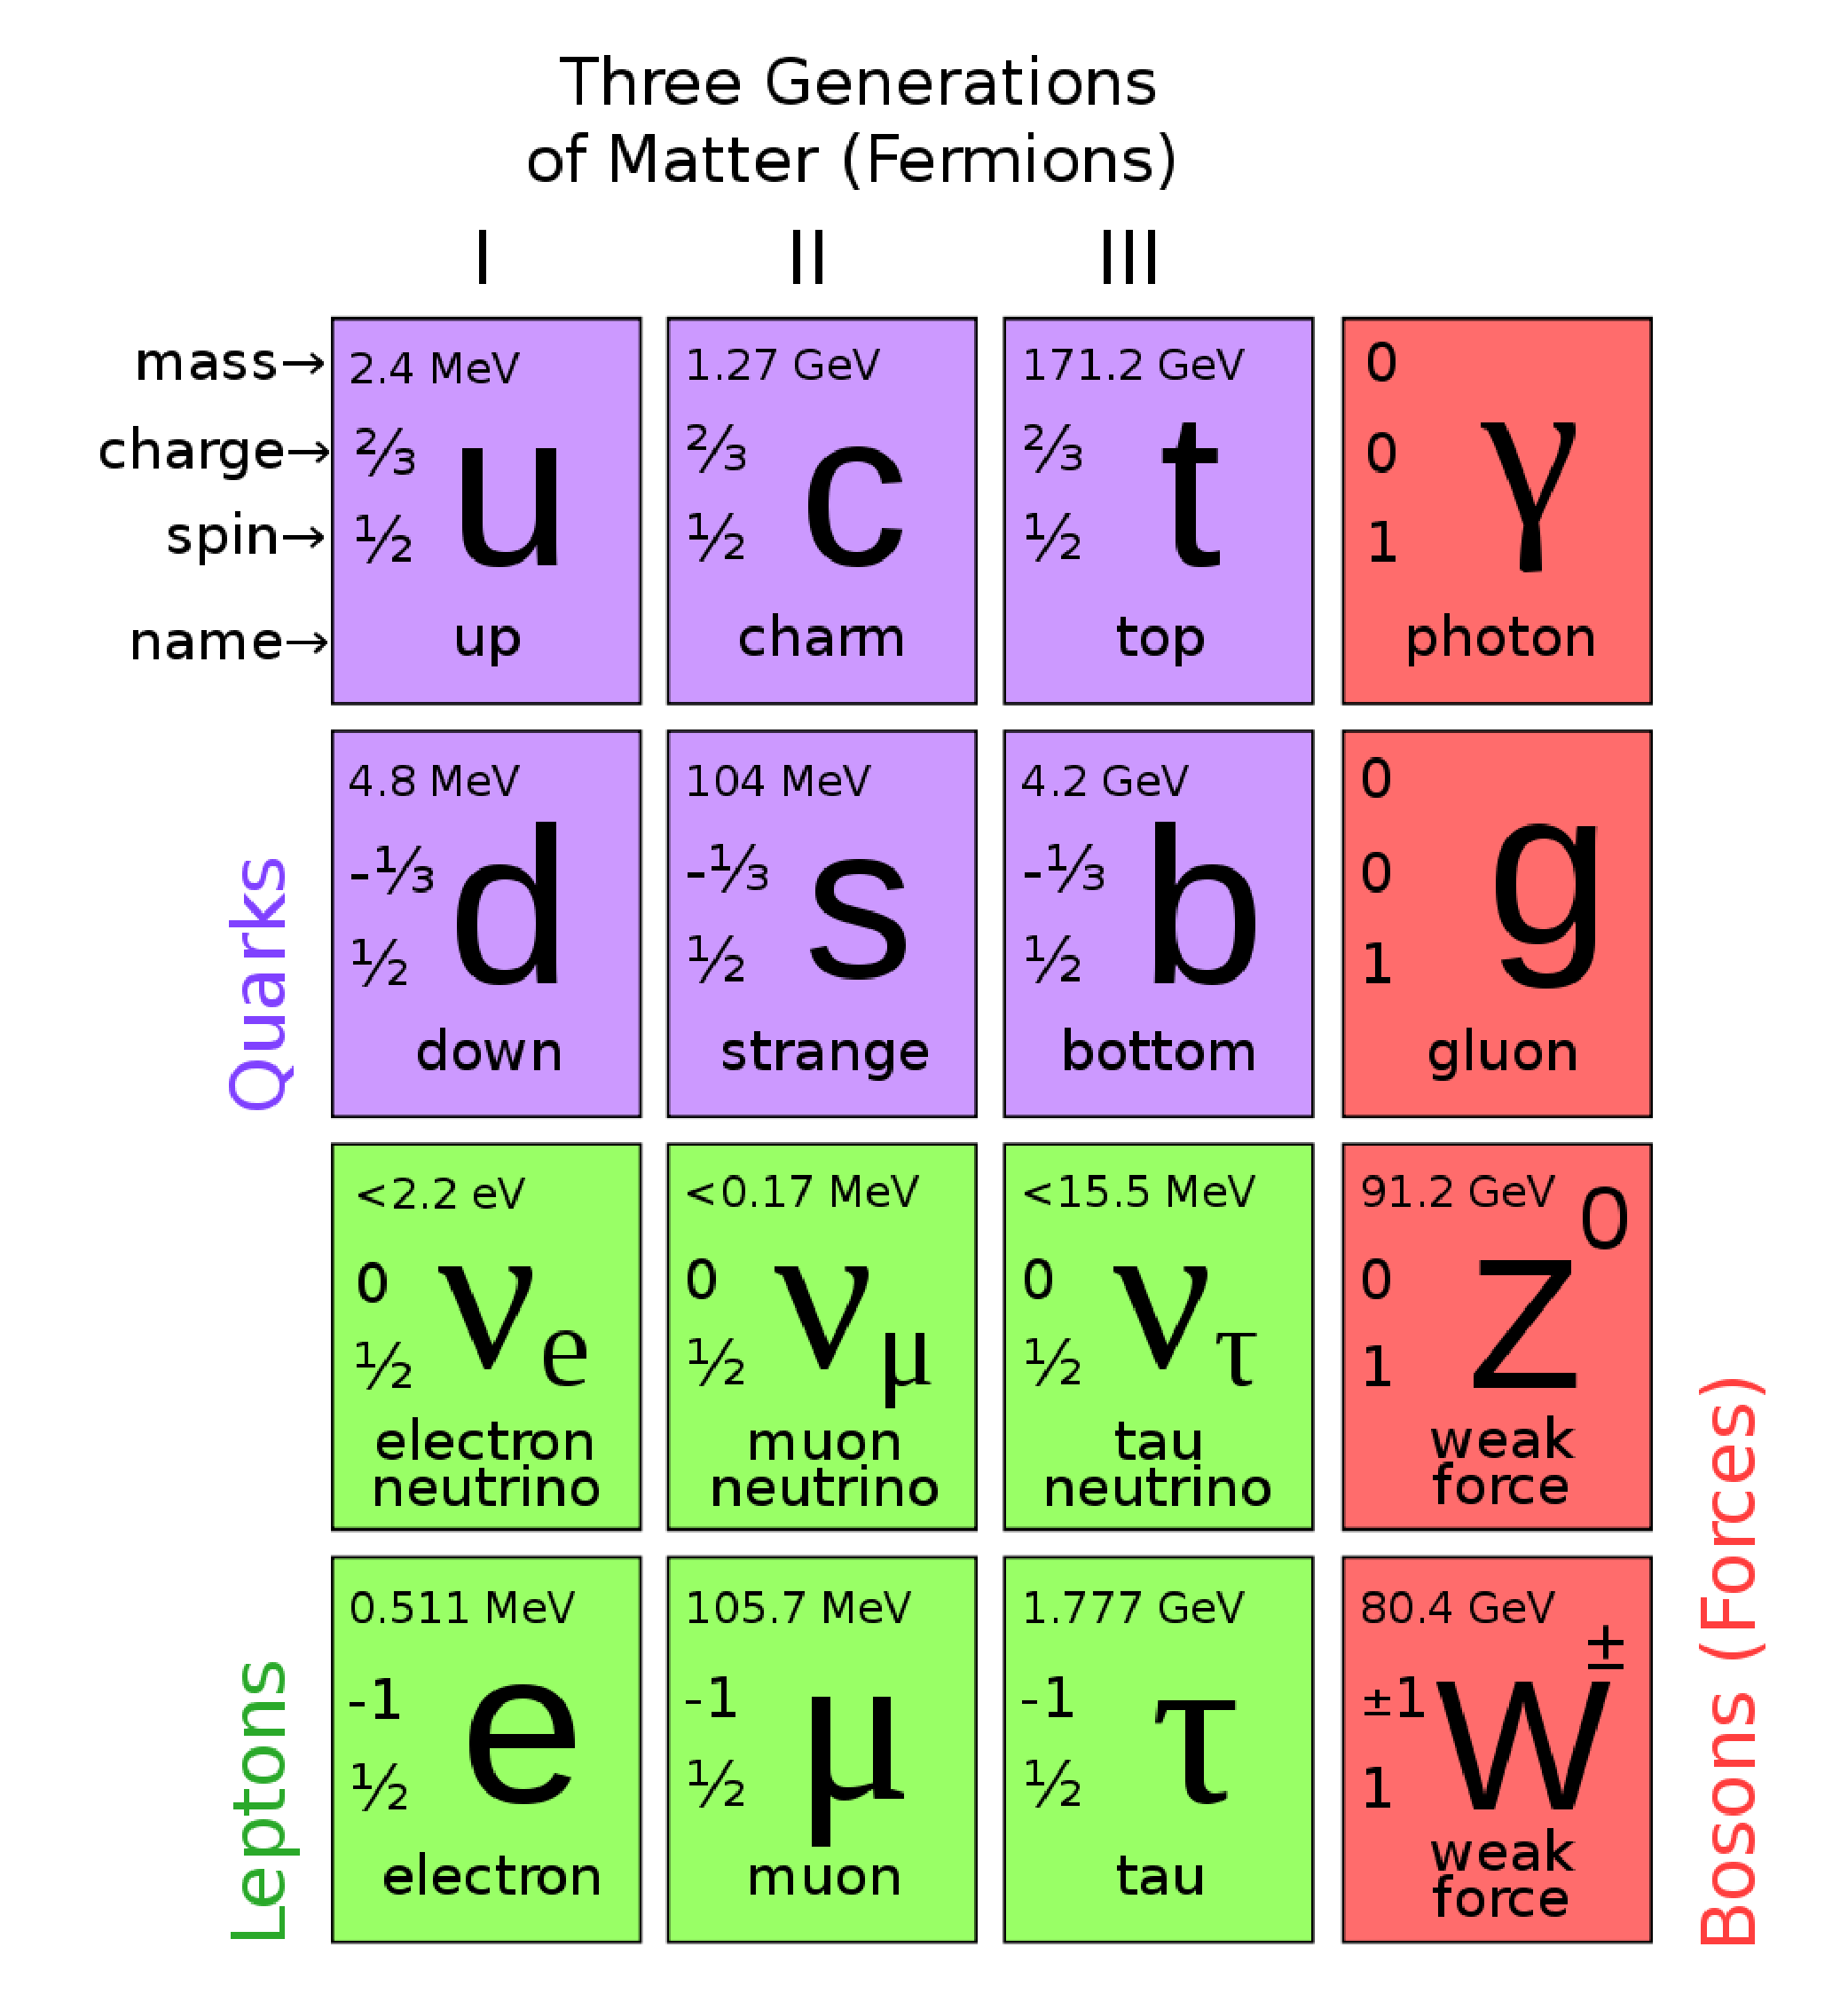
\includegraphics[width=.7\textwidth]{images/pdf/sm_particles}
    \caption{The particles in the unbroken SM.}
    \label{fig:sm_particles}
\end{figure}

\subsection{Spontaneous simmetry breaking: the Higgs mechanism}
We have only considered massless particles. This is not the case for all
the known fermions, and for the \W and \Z bosons. A mechanism was proposed
to preserve the gauge invariance of the lagrangian, while the vacuum state
is no longer a singlet under the action of the gauge group.

Spontaneous symmetry breaking of the local gauge symmetry in the SM provides massive
\W and \Z bosons and a new boson, called the Higgs boson.
In addition, we can obtain massive fermions by coupling them to the Higgs
field with Yukawa terms.

\subsection{The hierarchy problem}
Recently found evidence for a light Higgs boson, with a mass
near~\unit[125]{GeV}, are thought to be an indication of new symmetries and
new particles beyond the SM.

The theory predicts that the mass $m_H$ is subject to large radiative
corrections from loop diagrams similar to figure~\ref{fig:higgs_correction},
that should increase it by a large amount.
In the SM, fine tuning is required to prevent this corrections from becoming
too large. Theoretical physicists generally dislike this fine tuning on grounds of
\emph{naturalness}.

\begin{figure}[htb]
    \centering
    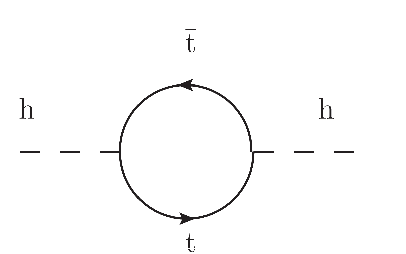
\includegraphics[width=.4\textwidth]{images/pdf/higgs_correction}
    \caption{Radiative correction to the Higgs mass from the top quark.}
    \label{fig:higgs_correction}
\end{figure}

The most notorious example of an extension to the SM that can eliminate this
naturalness problem is supersimmetry, where the radiative corrections to
the Higgs mass of the SM fermions are canceled by the contributions from
their superpartners.

There exist many theories that do not invoke supersimmetry as the solution
to the hierarchy problem. A robust and generic prediction of many of them is the
existence of new particles, the top partners, again balancing the
largest contribution to $m_H$ coming from the top quark.

\subsection{The top partners}\ref{sec:top_partner_theory}
Theoretical developments predicting the existence of top partners stem from
the search for a way of introducing gravity in the SM, while solving the
hierarchy problem at the same time.

Five-dimensional space-time theories including gravity can be formulated in
terms of effective 4-d lagrangians where SM quarks mix with the top
partners, which, again from arguments of naturalness, should have a mass below or
slightly above the \unit[]{TeV} scale.
The lightest quarks have a small mass, indicating that their mixing with the
new particles is negligible. The top quark, having a very large mass, should have
a sizeable mixing with its partner, possibly making deviation
from the SM top interactions detectable at the LHC.

We use the top partner model from~\cite{Mrazek:2009yu} to describe our
signal, with vertices with the vector bosons and the top quark. 
We study the possibility of observing the top partners in the very clean
channel of two same-sign hard leptons. Typical production and decay diagrams
are shown in figure~\ref{fig:T53_production}.

\begin{figure}[htb]
    \centering
    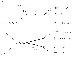
\includegraphics[width=\textwidth]{images/pdf/T53_production}
    \caption{Typical single and pair production the top partner $\TP$ at the
    LHC.}
    \label{fig:T53_production}
\end{figure}

\chapter{The LHC and the CMS detector}
\section{The Large Hadron Collider}
The LHC is a ring-shaped proton-proton accelerator with a circumference of
\unit[27]{km}. It is hosted in a tunnel 45 to \unit[170]{m} below ground at
the CERN laboratory in Geneva, Switzerland. In 2011, the LHC accelerated two
proton beams up to an energy of \unit[3.5]{TeV} each and an instantaneous
luminosity of up to $\unit[3.55\cdot 10^{33}]{cm^{-2}s^{-1}}$.

The two proton beams are pre-accelerated through four smaller systems before
being injected in the LHC:
\begin{itemize}
    \item the linear accelerator (up to \unit[50]{MeV})
    \item the proton synchrotron booster (up to \unit[1.4]{GeV})
    \item the proton synchrotron (up to \unit[26]{GeV})
    \item the super proton synchrotron (up to \unit[450]{GeV})
\end{itemize}

The protons travel in ultra-high vacuum around
$\unit[10^{-10}]{mbar}$, while different sets of magnets keep them in a
circular orbit and provide acceleration and focusing.

Radio frequency cavities in the LHC accelerate the protons, providing an energy
increase of $\unitfrac[0.5]{MeV}{turn}$.
Superconducting dipole magnets operate at currents of \unit[11850]{A} to bend the trajectories
of the protons with a magnetic field up to \unit[8.3]{T}.
Quadrupole magnets are employed to focus the beams, thus increasing the
probability of an interaction when they collide.
The magnets are cooled with superfluid helium at \unit[1.9]{K}.
The beams are made of ``bunches'' of protons with a time spacing of
\unit[75]{ns}.

At four different interaction points, the two proton beams are brought to
collision where the experiments are located: CMS, ATLAS, LHCb and ALICE, as
shown in figure~\ref{fig:lhc}.
The first two are general purpose detectors. LHCb is designed for the study
of CP violation in $\mathrm{b}$ physics, and ALICE for the analysis of the
quark-gluon plasma produced in heavy ion collisions.

\begin{figure}[htb]
    \centering
    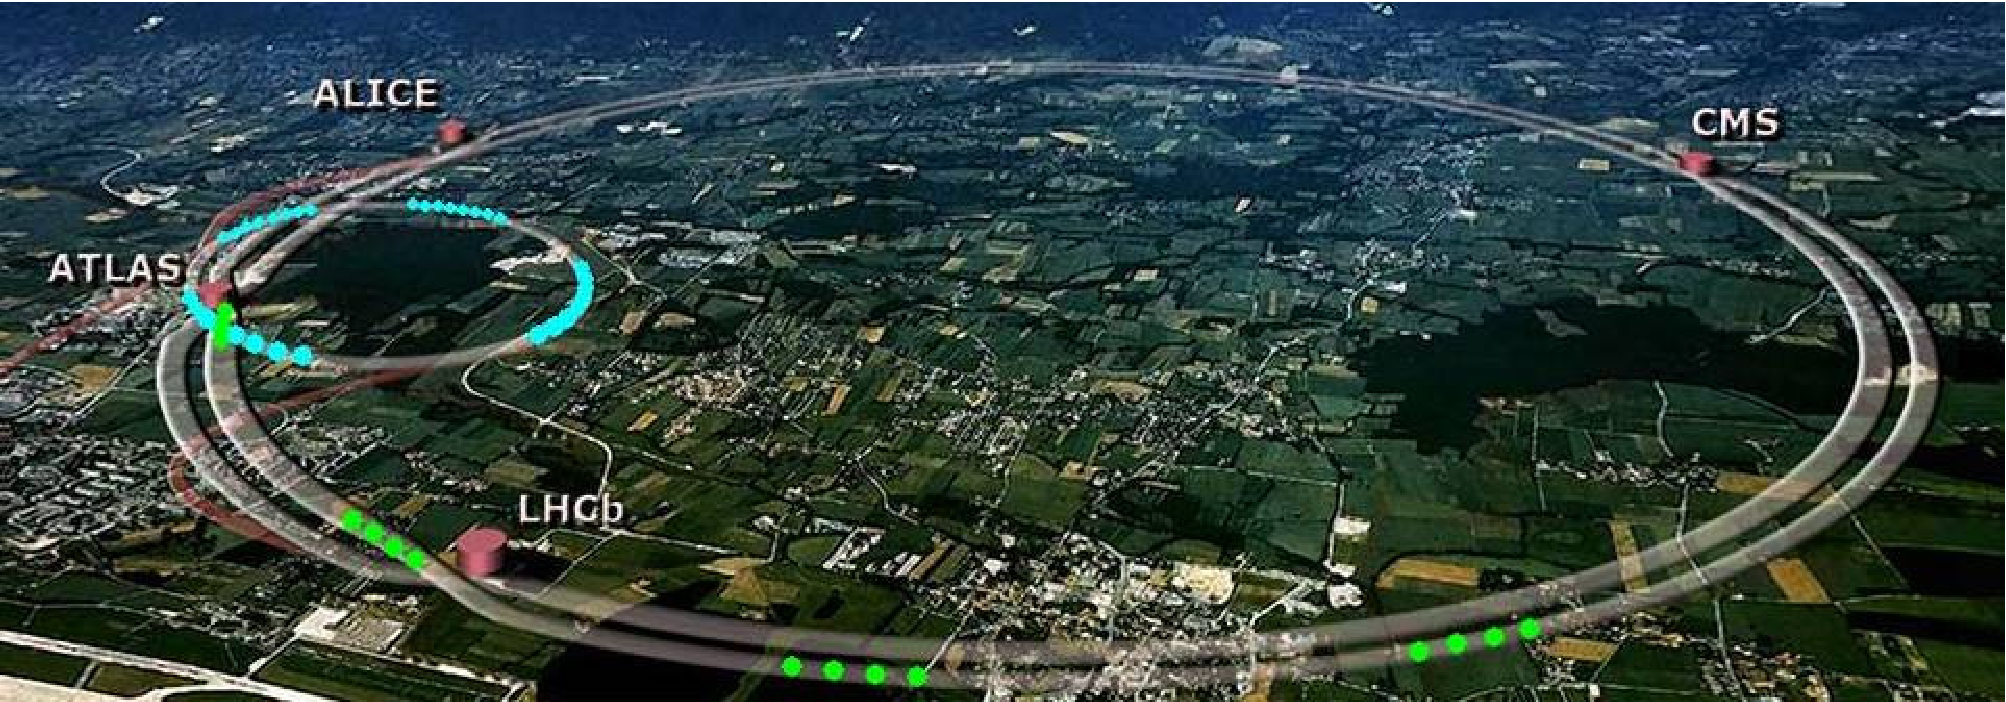
\includegraphics[width=\textwidth]{images/pdf/lhc}

    \caption{A view of the LHC and the four experiments.}
    \label{fig:lhc}
\end{figure}

\section{The Compact Muon Solenoid}
CMS is a general purpose detector based on interlocking cylindrical
subdetectors in the central \emph{barrel} region, closed by two
\emph{endcaps}, all placed coaxially with the beam and centred on the beam interaction point.
\subsection{Coordinate convention}
The conventional coordinate system has its origin at the nominal interaction
point. The $z$ axis points along the beam direction, the $y$ axis points
vertically upwards, and the $x$ axis points towards the centre of the LHC
circumference. The $xy$ plane is thus called the \emph{transverse} plane as
it is orthogonal to the CMS cylinder.

We define two angles in the transverse plane: the azimuthal $\varphi$ angle
is measured from the $x$ axis, and the polar angle $\theta$, measured from
the $z$ axis.
\emph{Pseudorapidity} is defined as $\eta = -\log \tan
\nicefrac{\theta}{2}$.

\subsection{Structure of the detector}
A global view and a transverse section of the detector are shown in
figures~\ref{fig:cms} and~\ref{fig:cms_transverse}.

\begin{figure}[htb]
    \centering
    \includegraphics[width=\textwidth]{images/pdf/cms}
    \caption{The CMS detector.}
    \label{fig:cms}
\end{figure}

\begin{figure}[htb]
    \centering
    \includegraphics[width=\textwidth]{images/pdf/cms_transverse}
    \caption{Transverse view of the CMS detector with some examples of tracks.}
    \label{fig:cms_transverse}
\end{figure}

A superconducting solenoid \unit[13.5]{m} and with a diameter of
\unit[5.9]{m} provides a uniform, axial magnetic field of \unit[3.8]{T}.
The return field saturates an iron yoke, which consists of five wheels in
the barrel region and three disks in each of the two endcaps.
Muon detectors are installed in the return yokes, with four stations of
aluminium drift tubes in the barrel and cathode strip chambers with
resistive plate chambers in the endcap.

The tracking system and the calorimeters are installed inside the solenoid.
The tracker is a cylinder with a diameter of \unit[2.6]{m} with three layers
of pixel detectors, allowing exceptional measurements of the impact parameter
of the particles and secondary vertex reconstruction, and ten layers of
silicon microstrip detectors.
The tracking system is surrounded by the calorimeters, which cover the
region with $|\eta| < 3$. There is an electromagnetic calorimeter (ECAL),
made of lead tungstate crystals and a brass/scintillator hadron calorimeter
(HCAL). A forward calorimeter provides additional coverage up to $|\eta| <
5$.

\subsection{The tracking system}
Very high granularity and time resolutions are needed in the tough
environment of the LHC experiments, with thousands of particles produced
for every interaction. The high spatial resolution is particularly important
in the region close to the primary interaction.

For these reasons, silicon detectors where chosen for the whole tracking
system of the CMS experiment.

\begin{description}
    \item[The pixel detector] is made of three cylinders in the barrel and
        two disks in each of the two endcaps. The spatial resolution on each
        hit is about \unit[10]{\micro m} in $r$-$\varphi$ and about
        \unit[20]{\micro m} in $z$.
    \item[The microstrip detector] is made of concentrical layers in the
        barrel region, divided in two systems: the \emph{tracker inner
        barrel} (TIB) and the \emph{tracker outer barrel} (TOB).

        The TIB has four layers in the region with $\unit[20]{cm} < r <
        \unit[55]{cm}$ and $|z| < \unit[65]{cm}$. The sensors are
        \unit[10]{cm} long in $z$, 80 to \unit[120]{\micro m} wide and
        \unit[320]{\micro m} thick. The single hit resolution is between 23
        and \unit[34]{\micro m} in the $r$-$\varphi$ plane, and about
        \unit[230]{\micro m} in $z$.

        The TOB module is made of six layers, covering
        $\unit[55]{cm} < r < \unit[116]{cm}$ and $|z| <
        \unit[116]{cm}$. The sensors have a length of \unit[25]{cm}, a width
        of \unit[180]{\micro m} and a thickness of \unit[500]{\micro m}. The
        single hit resolution is 35 to \unit[52]{\micro m} in the
        $r$-$\varphi$ coordinates, and \unit[530]{\micro m} in $z$.

        Two more modules are installed in the endcaps, arranged around the
        beam line: the \emph{tracker inner
        disks} (TID) and \emph{tracker outer endcaps} (TEC)

        Each TEC module consists of nine disks, while the TID have three
        smaller disks. Both these modules have strips pointing radially
        toward the beam line with a thickness of \unit[320]{\micro m} to
        \unit[500 \micro]{m}.
\end{description}

\subsection{The electromagnetic calorimeter}
The ECAL is the inner calorimeter, made of 61200 lead tungstate crystals in
the barrel and 7324 crystals in the endcaps.
The base of the crystals is about $\unit[2\times2]{cm}$ in size, with a
depth of $\unit[23]{cm}$, corresponding to 25 radiation lengths.

The scintillation light is collected by avalanche photodiodes in the barrel
and vacuum phototriodes in the endcaps. They have a high gain and are
insensitive to the magnetic field of the detector.

The energy resolution of the calorimeter has been measured in $\Z
\rightarrow \E\E$ events from the 2011 data~\cite{CMS-DP-2012-007}, as shown in
figure~\ref{fig:ecal_resolution}.

\begin{figure}[htb]
    \centering
    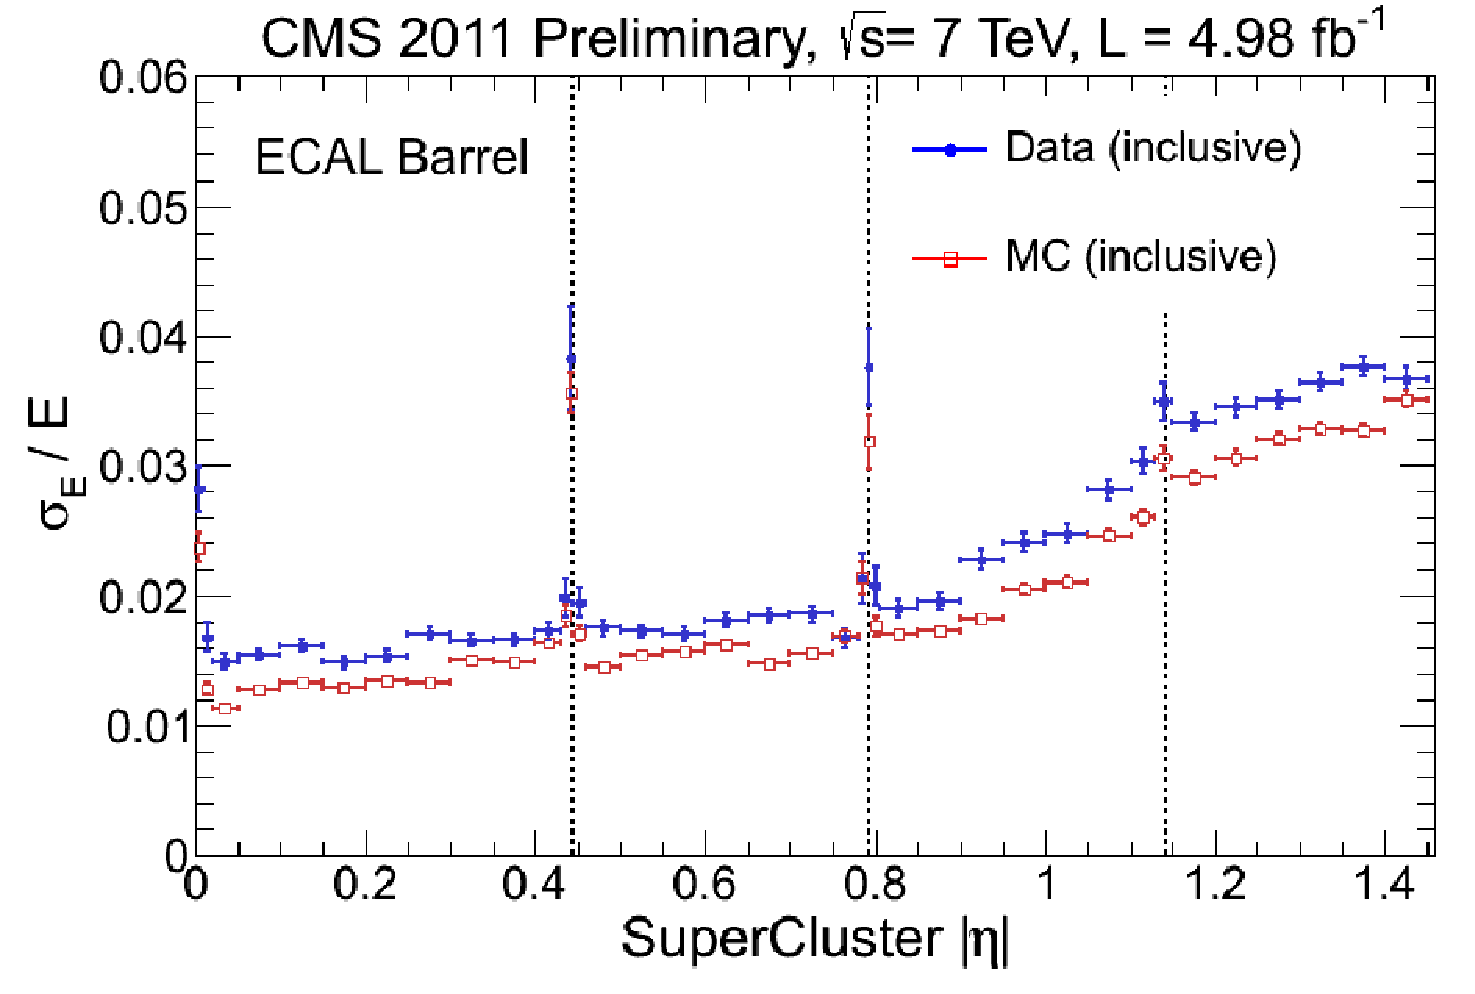
\includegraphics[width=.48\textwidth]{images/pdf/ecal_barrel_resolution}
    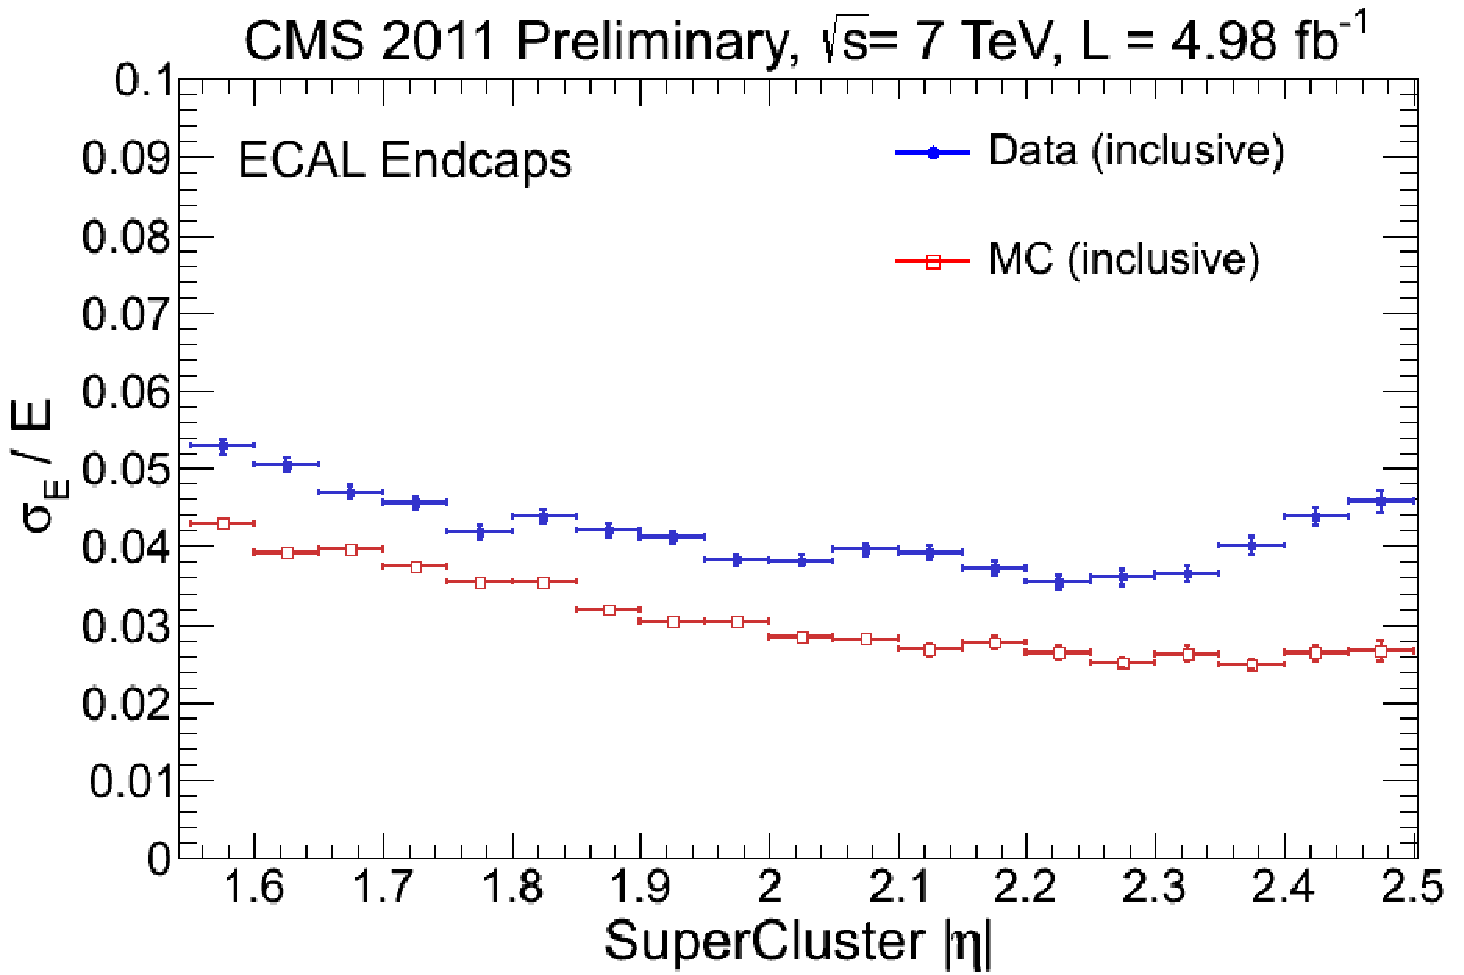
\includegraphics[width=.48\textwidth]{images/pdf/ecal_endcap_resolution}
    \caption{Energy resolution of the ECAL as measured in $\Z \rightarrow
    \E\E$ events in the 2011 data.}
    \label{fig:ecal_resolution}
\end{figure}

\subsection{The hadron calorimeter}
The HCAL surrounds the ECAL and is made of plastic scintillators interleaved with brass layers.
It is composed of a \emph{hadron barrel} up to $|\eta| < 1.4$, a
\emph{hadron endcap} for $1.3 < |\eta| < 3.0$. Two more systems provide
very good hermeticity: the \emph{hadron outer calorimeter} is placed
outside  the magnet in order to measure the energy of penetrating hadrons,
while the \emph{hadron forward calorimeter} extends the coverage up to
$|\eta| < 5$.

\subsection{The muon detectors}
The muon system is installed in the return yokes of the magnet. Concentrical
cylinders cover the barrel region up to $|\eta| < 1.2$, while four disks
make up the endcap detectors ($|\eta| < 2.4|$). Three kind of gas detectors
are employed: drift tubes in the barrel, cathode strip chambers id the
endcaps, and resistive plate chambers in both. This last kind of detector
has a fast response and is the most important for the trigger.

\begin{figure}[htb]
    \centering
    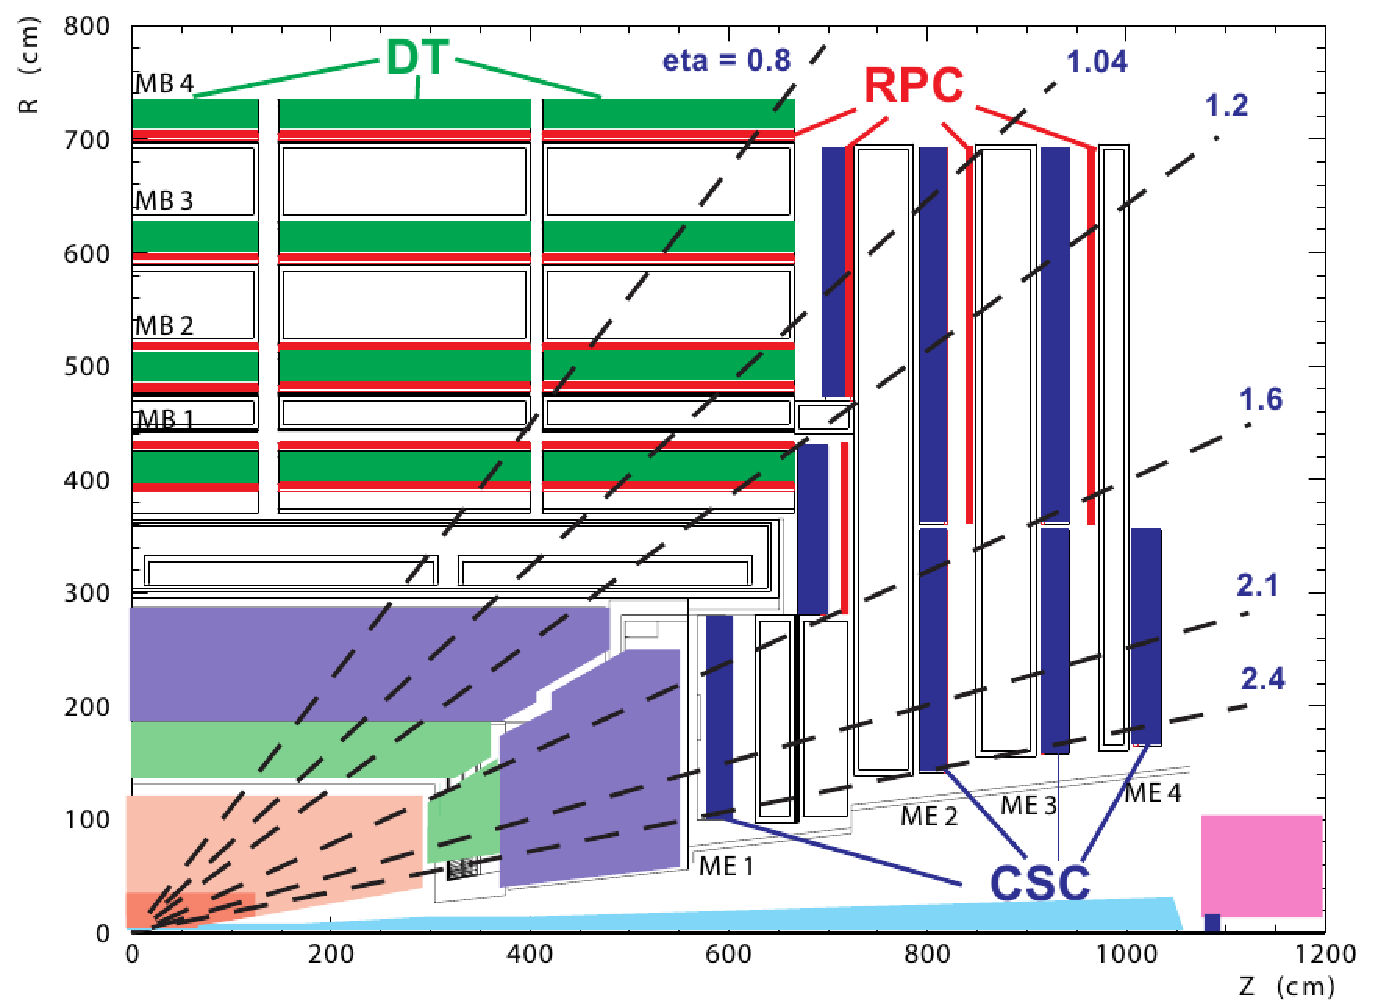
\includegraphics[width=\textwidth]{images/pdf/cms_muon_system}

    \caption{The layout of the muon detectors.}
    \label{fig:cms_muon_system}
\end{figure}

\subsection{The trigger and data acquisition system}
The design bunch spacing of the LHC is \unit[25]{ns}, \ie
\unit[40]{MHz}. About 100 interactions per second can be stored, so that
the trigger has to provide a reduction factor of the order of $10^{5}$.
The trigger system has two levels of selection: the \emph{level 1} (L1) and
the \emph{high level trigger}.
\begin{description}
    \item[L1] is a hardware trigger, made of processors close to the
        detector components. It exploits coarse granularity information from
        calorimeters and muon chambers to identify electromagnetic clusters,
        muons, jets and missing $E_t$. Its processing time per event is on
        the order of a microsecond. It reduces the rate of events to less
        than \unit[100]{kHz}.
    \item[HLT] is a software trigger run on a farm of commercial CPUs,
        and has access to all event data, allowing for precise object
        reconstruction and energy/momentum evaluation. The HLT processing
        time is around \unit[0.1]{s} per event.
\end{description}

\chapter{Simulation, reconstruction and datasets}
\section{Simulation}\label{sec:fast_sim}
Accurate Monte Carlo simulations are needed in order to make sense of the
data and search for new physics phenomena. The physics of the collisions is
simulated by the event generators MadGraph~\cite{madgraph} and PYTHIA~\cite{fs:pythia}. Then, the propagation of the particles in the detector has to be worked out.
Two different types of simulation are used by the CMS collaboration: a
GEANT4-based~\cite{fs:geant} simulation, known as the \emph{Full
Simulation}, and a detector model with simplified geometry, response
evaluation and pattern recognition to decrease the processing time per
event, the \emph{Fast Simulation}~\cite{fs:fast.simulation}. Both the
FullSim and the FastSim were employed in the generation of the background
samples for our studies.

In the FullSim, the energy depositions in the sensitive detector volumes are converted to electronic
signals using algorithms based on the observed detector behavior, including the simulation of
electronics noise and cross-talk. In many cases, the simulated electronic parameters are identical to
those of the real electronics; the constants specifying performance, calibrations, and noise behavior
can be read from the same database used for the reconstruction of the real collision data. The output of
this stage is simulated data in a format identical to that of the real raw data read from the detector.
Further processing uses this data to simulate the formation of the L1 and
HLT decisions using the same algorithms implemented online in the CMS trigger system. The simulated
raw data that is produced is processed in a manner identical to that of the real data from
LHC collisions.

The FastSim makes a number of approximations:
\begin{description}
    \item[CMS geometry:] the FastSim describes the detector with a simplified geometry of nested cilyndrical layers. The particles are propagated from one layer to the next.
    \item[Material effects:] five effects are taken into account. These are \emph{bremsstrahlung}, photon conversion, multiple Coulomb scattering, energy loss through ionization and nuclear interactions. All of these are calculated analytically, except for nuclear interactions, since no analytical description is sufficient to describe the effect. Cross sections are taken from the PDG and the kinematics are derived from single particle collisions saved beforehand.
    \item[Track reconstruction:] the reconstruction is not usually part of the simulation. The FastSim includes it because, given the low fake rate in the reconstruction, it is possible to emulate it at a lower computational cost. Only the hits of the simulated track are used to make a track candidate. 
    \item[Muons:] muons are propagated through the tracker and calorimeters with average energy loss, then $dE/dx$ and multiple scattering in the iron yokes of the muon chambers are computed. Muon simulated hits are produced in all sections of the muon systems.
    \item[Calorimeters:] electron showers in the ECAL are simulated with the Grindhammer~\cite{fs:grindhammer} parametrization. Photons undergo pair conversions based on the number of radiation lengths they have traversed. Detector effects such as energy leakage into the crystal gaps and into the HCAL are included, as well as electronic noise. Shower simulation in the HCAL is similar, with different types of particles parametrized from FullSim results.
\end{description}

\section{The reconstruction of physics objects}
The particle flow~\cite{pf:particle.flow} (PF) event reconstruction aims at reconstructing and identifying all stable particles in the event. The essential idea is to analyse the event combining the information from all the available subdetectors in an optimal way.

The CMS detector, with its large silicon tracker and its extremely precise electromagnetic calorimeter, appears to be ideally suited for this purpose. The fundamental building bricks of the PF reconstruction are charged particle tracks, ECAL and HCAL clusters and muon tracks. These must be delivered with a high efficiency and low fake rate even in high-density environments like jets. A jet is a collection of particles resulting from the decay of a quark or gluon and emitted in the direction of the primary particle. 

Reconsider the design of the detector in figure~\ref{fig:cms_transverse}. The logic you use to
interpret this diagram is akin to that employed by the PF.
An ECAL cluster not linked to any track is a photon, an ECAL and HCAL cluster matched to a track gives a charged hadron, while an HCAL cluster without a track identifies a neutral hadron. Electrons are basically ECAL-only clusters linked to a track. Muons are by far the easiest particles to recognize.

From these basic elements, composite objects can be reconstructed, such as
$\tau$ leptons from their decay products, jets and
missing transverse energy from all the particles in the event.

Quality requirements are needed in the reconstruction of the physics
objects: thousands of particles are created in each event and their tracks
can overlap.
The quality selections are the result of detailed studies by the CMS
collaboration, aiming for the best compromise between purity and efficiency.
These recommendations are described in the following paragraphs.

\subsection{Muon reconstruction}
Muons are not stopped inside the CMS detector and leave only a tiny fraction
of their energy in the calorimeters. The information from the tracking
system and the muon chambers is exploited for their reconstruction.
The two systems are used independently in a first phase, where two
algorithms are used:
\begin{description}
    \item[The global muon reconstruction], or the \emph{outside-in}
        approach, starts from a segment in the drift tubes or cathode strip
        chambers and extrapolates the seed layer by layer up to the
        tracker. If a matching track is found in the tracking system, the
        information from both tracks is combined to improve the resolution.
    \item[The tracker muon reconstruction], or the \emph{inside-out} method,
        extrapolates a track from the inner system to the muon chambers. The
        small energy loss due to interactions with the material of the
        magnets and calorimeters is taken into account, as well as an
        uncertainty arising from the possibility of multiple scattering.
\end{description}
The recommended selection requires these two algorithms to agree, as this
improves the resolution for high-$\pt$ muons
(figure~\ref{fig:muon_resolution}).

\begin{figure}[htb]
    \centering
    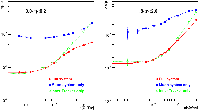
\includegraphics[width=\textwidth]{images/pdf/muon_momentum_resolution}
    \caption{Muon momentum resolution as a function of \pt in regions with
    different pseudorapidity. The blue squares are for the muon system only,
the green circles for the inner tracker only, and the red circles for the
combined reconstruction}
    \label{fig:muon_resolution}
\end{figure}

One of the most important observables for the muon candidates is the
\emph{relative isolation}. It indicates the amount of energy collected in
the vicinity of the muon, by summing the contributions from the tracking
system, the ECAL and the HCAL, divided by the \pt of the muon.
The sum runs over all deposits within a cone of radius $\Delta R = 0.3$
centred on the muon track, as illustrated in figure~\ref{fig:muon_isolation}.

\begin{figure}[htb]
    \centering
    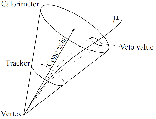
\includegraphics[width=.5\textwidth]{images/pdf/muon_isolation}
    \caption{Illustration of the isolation observable.}
    \label{fig:muon_isolation}
\end{figure}

\subsection{Electron reconstruction}\label{sec:electron_reco}
The tracks in CMS are reconstructed assuming that the particle is a muon.
Coulomb scattering is the dominant effect on muons crossing material and its
impact is modelled by gaussian fluctuations. This approach fails with
electrons because of the highly non-gaussian \emph{bremsstrahlung} emission. A
customized track reconstruction was developed for electrons, where the hits
are fitted using a \emph{gaussian sum filter} (GSF)~\cite{pf:gsf.tracks},
\ie the \emph{bremsstrahlung} emission is modelled by a superposition of
gaussian functions. However, this more sophisticated analysis demands more CPU power, at the order of a few hundreds milliseconds per track, and can be run only on a limited number of seeds.

The standard strategy to seed GSF tracks, hereafter called ECAL-driven seeding, heavily relies on
the ability to gather into one single \emph{supercluster} the entire energy deposit of the electron. 
The algorithm consists of three steps. First, cluster seeds are identified
as local energy maxima above a given energy. Secondly, the seeds are
grown by connecting cells with at least one side in common with
a cell already in the cluster, and with an energy in excess of a given
threshold. These thresholds are equivalent to two standard deviations of the electronic noise in the calorimeter, that is $\unit[80]{MeV}$ in the ECAL barrel, up to $\unit[800]{MeV}$ in the HCAL. Finally cluster energies and positions are determined from those clusters.

This implies collecting the electron and the \emph{bremsstrahlung} photons energy deposits, 
which leads to clusters very extended along the azimuthal direction. 
This approach, which is efficient for isolated and high $\pt$ electrons has unfortunately 
a limited efficiency in jets because the super-cluster collects 
additional contributions from other particles.

In contrast with this ECAL-driven approach, the strategy developed for the Particle Flow~\cite{pf:electron.reconstruction} starts from
the tracks and can be explained with two extreme examples. 
When the \emph{bremsstrahlung} emission is negligible, the electron
trajectory is determined with good precision by
the standard tracking algorithm, and the track can be reconstructed up to the ECAL internal
surface where it can be matched with the closest cluster. 
The momentum of the track can then be compared with the corresponding cluster energy, 
forming the $E/p$ observable. If it is close to unity the track is selected to be then re-reconstructed
with the GSF algorithm. On the contrary, if the electron loses a substantial fraction of its energy by \emph{bremsstrahlung} emission, the characteristics of the track are exploited. Indeed, either the pattern recognition manages
to accommodate for the changes of curvature, and the fitted track $\chi^2$ is usually large, or
it cannot follow the electron trajectory and the track is short.  
Electron tracks are then selected based on the attempt made by the standard algorithm to reconstruct it. 

The tracker-driven seeding developed for the PF reaches a 80\% efficiency in the barrel with a 10\% probability
to select wrongly a pion, with an acceptable CPU consumption; a more sophisticated treatment described below 
is further applied to reject fakes at the final identification level. 
In addition, this new algorithm improves the overall seeding efficiencies for isolated electron in CMS by 15\% at \unit[5]{GeV} with respect to the standard ECAL-driven seeding. 

\begin{figure}[htb]
    \centering
    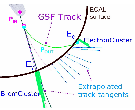
\includegraphics[width=.5\textwidth]{images/pdf/electron_reconstruction}

    \caption{An illustration of the \emph{bremsstrahlung} recovery
algorithm.}
    \label{fig:electron_reconstruction}
\end{figure}

The procedure to collect all the calorimeter energy deposits, \ie, the \emph{bremsstrahlung} recovery, is
driven by the GSF track (figure~\ref{fig:electron_reconstruction}). For each tracker layer, where 
the material is mainly localized, a \emph{bremsstrahlung} photon emission is sought by computing a straight-line
extrapolation, tangent to the track, up to the ECAL. If it matches a cluster, not already linked
to a track, this cluster is selected as part of the electron. 
This procedure allows between 96\% and 99\% of the energy deposited in the ECAL to be collected.

The relative isolation is defined with the same method already described for
the muons.

The charge of the electrons can be measured in three ways:
\begin{description}\label{page:electron_charge}
    \item[The GSF track] whose curvature in the magnetic field of the
        detector defines the sign of the charge of the electron.
    \item[The CTF track] algorithm for the reconstruction of the
        tracks. It accounts for multiple scattering with Kalman filter
        techniques~\cite{springerlink:10.1140/epjc/s10052-006-0175-5}. The
        curvature of this track is another measurement of the charge.
    \item[Supercluster relative position] the relative position of the track seed
        and the largest deposition in the ECAL provides an indipendent
        estimate of the electric charge.
\end{description}
Requiring these three methods to agree strongly decreases the probability of
a charge mismeasurement. This is particularly important for our analysis,
since the production of opposite-sign electrons is very abundant in Standard
Model processes, and the accurate identification of the charge of the
electrons almost eliminates these contributions.

Electrons can also be created from the conversion of an energetic photon.
These are rejected if one of the following occurs:
\begin{description}
    \item[At least one missing hit] in the tracker. Photons are neutral, so they
        usually miss hits in one or more layers.
    \item[Track distance] $< \unit[0.02]{cm}$. An electron coming from a
        conversion has a partner positron track. If an oppositely charged
        track is found within this distance, the electron is rejected.
    \item[$\Delta \cot \theta < 0.02$]. A geometrical variable also related
        to the partner track: $\theta$ is the angle between the two tracks
        in the $yz$ plane.
\end{description}

\subsection{Jet reconstruction}\label{sec:jet_reco}
A quark or gluon produced in the hard scattering process undergoes
hadronization due to colour confinement. Many hadrons are created, mostly in
the same direction of the original parton, because of momentum conservation.
All of these collimated particles form a jet.

However there can be difficulties in collecting all the particles in a jet:
\begin{itemize}
    \item two or more jets may overlap, resulting in ambiguities in the assignment of the particles
    \item particles could be generated with a large momentum relative to the
        original parton direction, leading to the particle not being counted
        in the jet
    \item pile-up and initial state radiation may contribute with additional
        tracks 
\end{itemize}
The anti-$k_T$ algorithm~\cite{antikt} is used for the jet reconstruction. In this
algorithm the distances between the particles $i$ and $j$ $d_{ij}$ are defined, as well
as the distance between the $i$th-particle and the beam $d_{iB}$:
\begin{align*}
    d_{ij} &= \min(p_{Ti}^{-2}, p_{Tj}^{-2})\dfrac{\Delta_{ij}}{R^2}\\
    d_{iB} &= p_{Ti}^{-2}
\end{align*}
Where $\Delta_{ij}^2 = (y_i - y_j)^2 + (\varphi_i - \varphi_j)^2$, and
$p_{Ti}$, $y_i$ and $\varphi_i$ are the transverse momentum, rapidity and
azimuthal angle of the $i$th particle; $R = 0.5$ is a parameter representing a
typical radius of the jet.

The algorithm then compares $d_{ij}$ and $d_{iB}$ iteratively:
\begin{itemize}
    \item if $d_{ij} < d_{iB}$ for some $j$, $i$ and $j$ are merged into the
        same jet candidate
    \item if $d_{ij} > d_{iB}$ for all $j$, then $i$ is a jet.
\end{itemize}

After the jets have been reconstructed, the energy has to be scaled to
account for possible mismeasurements~\cite{2011JInst...611002C}. The following corrections
are used in this analysis:
\begin{description}
    \item[charged hadron subtraction:] charged hadrons originating from a
        secondary vertex are eliminated from the collection of particles
        in the jet reconstruction algorithm
    \item[Level 1 correction:]removes the energy coming from pile-up
        events. In principle this will removes any dataset dependence on luminosity so that the following corrections are applied upon a luminosity independent sample.
    \item[Level 2 correction:] makes the response independent from
        $\eta$, by using correction factors determined in dijet events.
    \item[Level 3 correction:] makes the response independents from the \pt
        of the jet. The correction factors are calculated from $\Z/\gamma +
        \text{jets}$ events.
    \item[L2L3 residual corrections:] are only applied to the data, and not
        to Monte Carlo samples. This fixes the small differences between the
        data and Monte Carlo reconstructions, in a \pt and $\eta$ dependent
        fashion.
\end{description}
The same corrections can be applied to the MC and data because of the very
high quality of the simulation. The residual corrections account for the
small difference.
The recommendations from~\cite{an:jetid} are also applied, by selecting jets
with:
\begin{itemize}
    \item neutral hadron fraction $< 0.99$
    \item charged hadron fraction $< 0.99$
    \item number of constituents $> 1$
\end{itemize}

\subsubsection{Jet b-tagging}\label{sec:btagging}
The signal features two b quarks in the final state of each event. Many
techniques have been developed to identify jets originated by a b quark. In
this analysis, the \emph{combined secondary
vertex} algorithm~\cite{CMS-PAS-BTV-09-001} is used. This sophisticated and complex tag exploits all known variables, which can distinguish b from non-b jets. Its goal is to provide optimal b-tag performance, by combining information about impact parameter significance, the secondary vertex and jet kinematics.
The standard \emph{loose} working point of this algorithm is employed, leading to a
a probability of a light-flavour jet passing this selection to 10\%,
as measured on jets with \pt of about \unit[80]{GeV} in QCD Monte Carlo
events~\cite{CMS-PAS-BTV-11-001}.

\section{Object selection}
Signal events in our studies have a clean signature: two clean, isolated,
same-sign leptons and many jets. To reduce the probability of pions and
other objects of being wrongly identified as leptons further quality
requirements are enforced.
\subsection{Muon selection}\label{sec:muon_selection}
The muons considered for our analysis have the following properties, mainly
concerning the quality of the reconstructed track, besides high \pt and
isolation:
\begin{itemize}
    \item $\pt > \unit[30]{GeV}$
    \item relative isolation $< 0.20$
    \item $|\eta| < 2.4$
    \item reconstructed as global and tracker muon
    \item at least eleven silicon hits
    \item transverse impact parameter $< \unit[0.02]{cm}$
    \item normalized $\chi^2 < 10$
    \item at least one hit in the muon system
    \item at least one hit in the pixel detectors
    \item at least two muon chambers whose track segments match
\end{itemize}

\subsection{Electron selection}\label{electron_selection}
The selection of electron candidates is more complex due to the high
material budget in the CMS detector and high magnetic field. More variables are
needed to achieve good discriminating power against fakes.
The CMS collaboration studied the following variables for electron
identification:
\begin{description}
    \item[tracker-ECAL matching,] with $\Delta \varphi$, $\Delta \eta$ and
        $E/p$ between the track reconstructed in the silicon detector and
        the ECAL energy deposits being compared
    \item[hadron fraction] $H/E$, where the energy collected in the HCAL
        directly behind the ECAL cluster is measured
    \item[cluster shape] in $\eta$
    \item[impact parameter]  with respect to the primary vertex
    \item[conversion rejection] with missing hits and partner track
        matching, as described in paragraph~\ref{sec:electron_reco}
    \item[isolation] of the electron in the tracker, ECAL and HCAL
\end{description}
The algorithm gives as output a selection for each electron candidate for
nine defined severity levels. In this analysis, the \texttt{HyperTightMC1}
level is used. The efficiency and fake rate of this selection are shown in
figures~\ref{fig:hyper_tight_efficiency}
and~\ref{fig:hyper_tight_fake_rate}.

\begin{figure}[htb]
    \centering
    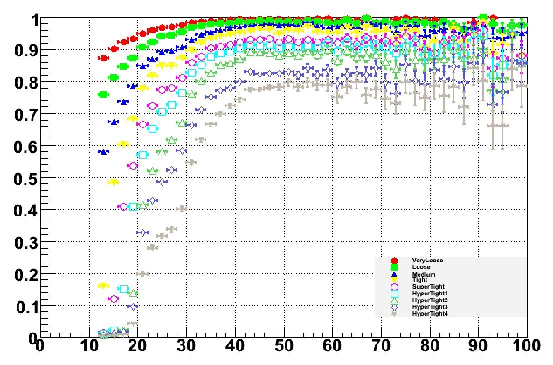
\includegraphics[width=\textwidth]{images/pdf/hyper_tight_efficiency}
    \caption{Selection efficiency for the various working points, measured
    in $\Z \rightarrow \E \E$ and $\W \rightarrow \E \Nu$ events. In this
    analysis the \texttt{HyperTightMC1} selection (light blue squares) is used.}
    \label{fig:hyper_tight_efficiency}
\end{figure}
\begin{figure}[htb]
    \centering
    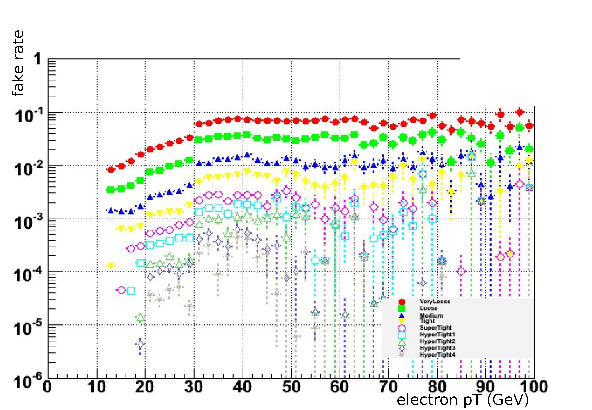
\includegraphics[width=\textwidth]{images/pdf/hyper_tight_fake_rate}
    \caption{Selection fake rate for the various working points, measured
    in QCD dijet events. In this
    analysis the \texttt{HyperTightMC1} selection (light blue squares) is used.}
    \label{fig:hyper_tight_fake_rate}
\end{figure}

Our final electron selection includes:
\begin{itemize}
    \item $\pt > \unit[30]{GeV}$
    \item relative isolation $< 0.15$
    \item $|\eta| < 2.4$, also excluding the transition region from the
        barrel to the endcap in the ECAL, with $1.444 < |\eta| < 1.566$.
    \item \texttt{HyperTightMC1} category
    \item conversion rejection
    \item transverse impact parameter $< \unit[0.02]{cm}$
    \item GSF-CTF-SC charge consistency (see
        paragraph~\ref{sec:electron_reco})
    \item $\Delta R > 0.1$ from all muon tracks. It can happen that a muon
        track matches by chance with an ECAL energy deposit. It is
        particularly important for the counting of $\E \M$ events that we remove such fakes.
\end{itemize}

\subsection{Jet selection}
The jet selection has only few requirement in addition to the baseline
reconstruction described in~\ref{sec:jet_reco}:
\begin{itemize}
    \item $\pt > \unit[30]{GeV}$
    \item $|\eta| < 2.4$
    \item $\Delta R > 0.3$ between the jet and the selected leptons, to
        avoid double counting the leptons as jets.
\end{itemize}

\subsection{Event cleanup and vertex selection}\label{sec:event_cleanup}
A pre-selection for the events includes some requirements on the quality of
the overall reconstruction:
\begin{itemize}
    \item the event is rejected if the fraction of high-purity tracks if
        less than \nicefrac{1}{4} in events with at least ten tracks
    \item at least one primary vertex, with at least four degrees of freedom
        and $\Delta z < \unit[24]{cm}$, $\Delta r < \unit[2]{cm}$ with
        respect to the nominal interaction point
    \item events with high levels of noise in the HCAL are removed
\end{itemize}

\subsection{Trigger requirements}\label{sec:triggers}
HLT selections are also used in our analysis. Double lepton triggers are
employed with a relatively high \pt threshold. The triggers used for the
three decay channels are listed in table~\ref{tab:triggers}.
\begin{table}[htb]
\small{
\begin{tabular} {ll}
    \toprule
HLT\_DoubleMu7\_v1,2 or \\
HLT\_Mu13\_Mu8\_v2,3,4,6,7 or \\
HLT\_Mu17\_Mu8\_v10,11 \\
\midrule
HLT\_Ele17\_CaloIdL\_CaloIsoVL\_Ele8\_CaloIdL\_CaloIsoVL\_v1,2,3,4,5,6 or \\
HLT\_Ele17\_CCTT\_Ele8\_CCTT\_v6,7,8,9,10 \\
\midrule
HLT\_Mu10\_Ele10\_CaloIdVL\_v2,3,4,or \\
HLT\_Mu17\_Ele8\_CaloIdVL\_v1,2,3,4,5,6,8 or \\
HLT\_Mu17\_Ele8\_CaloIdT\_CaloIsoVL\_\_v4,7,8 or \\
HLT\_Mu8\_Ele17\_CaloIdL\_v1,2,3,4,5,6 or \\
HLT\_Mu8\_Ele17\_CaloIdT\_CaloIsoVL\_v3,4,7,8 \\
\bottomrule
\end{tabular}
}
\caption{List of triggers used in the analysis.}
\label{tab:triggers}
\end{table}


\section{Datasets}
This analysis used the data recorded in 2011 at the CMS detector,
corresponding to an integrated luminosity of $\unit[5.0]{fb^{-1}}$ of
proton-proton collisions at a centre of mass energy of
$\sqrt{s}=\unit[7]{TeV}$.
The data is divided into \emph{runs} in which the beam and detector
conditions are stable. The runs are further divided into
\emph{lumisections}, corresponding to about \unit[23]{s}.

The CMS collaboration certifies a list of good runs based on the conditions
of the detector. This work is based on the official list of \emph{golden}
runs for physics analyses.

To enable the most effective access to CMS data, the data are first split
into \emph{primary datasets} (PDs). The division into PDs is done based on the trigger decision.
The datasets used in this analysis are triggered with a pair of leptons and
they are shown in table~\ref{tab:data_pd}.

\begin{table}[htb]
\centering
\begin{tabular}{ll}
    \toprule
Dataset & Run range  \\  
\midrule
/DoubleMuon/Run2011A-May10ReReco-v1/AOD & 160329-163869\\
/DoubleMuon/Run2011A-PromptReco-v4/AOD & 165071-168437 \\
/DoubleMuon/Run2011A-05AugReReco-v1/AOD & 170053-172619\\
/DoubleMuon/Run2011A-PromptReco-v6/AOD & 172620-175770\\
/DoubleMuon/Run2011B-PromptReco-v1/AOD & 175832-180296\\

/DoubleElectron/Run2011A-May10ReReco-v1/AOD & 160329-163869\\
/DoubleElectron/Run2011A-PromptReco-v4/AOD & 165071-168437 \\
/DoubleElectron/Run2011A-05AugReReco-v1/AOD & 170053-172619\\
/DoubleElectron/Run2011A-PromptReco-v6/AOD & 172620-175770\\
/DoubleElectron/Run2011B-PromptReco-v1/AOD & 175832-180296\\

/MuEG/Run2011A-May10ReReco-v1/AOD & 160329-163869\\
/MuEG/Run2011A-PromptReco-v4/AOD & 165071-168437 \\
/MuEG/Run2011A-05AugReReco-v1/AOD & 170053-172619\\
/MuEG/Run2011A-PromptReco-v6/AOD & 172620-175770\\
/MuEG/Run2011B-PromptReco-v1/AOD & 175832-180296\\
\bottomrule
\end{tabular}
\caption{Data samples used for the analysis.}
\label{tab:data_pd}
\end{table}


\section{Signal Monte Carlo samples}
The model described in~\ref{sec:top_partner_theory} has been implemented in
the MadGraph event generators and eight samples corresponing to values of
the \TP mass from 400 to \unit[750]{GeV} were generated. In these samples,
two of the same-sign \W bosons arisind from the decay of the top partners
were forced to decay leptonically. The approximate next-to-next-to-leading
order cross sections were calculated using HATHOR~\cite{hathor}. The masses,
cross sections and the number of generated events for the eight mass points
are listed in table~\ref{tab:signal_mc}. 

\begin{table}[htb]
    \centering
    \begin{tabular}{*4c}
        \toprule
        \unit[mass]{(GeV)} & \unit[$\sigma \times \text{BR}$]{(pb)} & events \\
        \midrule
        400 & 0.295 & 86205 \\
        450 & 0.139 & 86211 \\
        500 & 0.069 & 86684 \\
        550 & 0.036 & 86724 \\
        600 & 0.019 & 86965 \\
        650 & 0.011 & 87592 \\
        700 & 0.006 & 88145 \\
        750 & 0.004 & 88410 \\
        \bottomrule
    \end{tabular}
    \caption{Signal Monte Carlo samples. The branching ratio is 0.21.}
    \label{tab:signal_mc}
\end{table}


\section{Background Monte Carlo samples}
Some rare Standard Model processes also produce isolated, same-sign leptons
in their final state. These include the production of two or more vector
bosons, $\W\Z$, $\Z\Z$, $\W^\pm\W^\pm$ and $\W\W\W$, and the production of
a top-antitop pair with an associated vector boson, $\ttbar W$ and
$\ttbar \Z$. Some of them were not available in the official productions
from the CMS Collaboration and were privately produced with the Fast
Simulation of the detector, described in paragraph~\ref{sec:fast_sim}.

The background samples used in this analysis are listed in
table~\ref{tab:background_mc}.

\begin{table}[phtb]
    \centering
\begin{tabular}{llrr}
    \toprule
process & MC generator & \unit[$\sigma$]{(pb)} & events \\
\midrule
$\W\Z+$Jets                                          & MADGRAPH & 0.879 & 1221134  \\
$\Z\Z+$Jets                                          & MADGRAPH & 0.076 & 1185188  \\
$\W^{+}\W^{+}+$Jets                                  & MADGRAPH & 0.165        & 130000    \\
$\W^{-}\W^{-}+$Jets                                  & MADGRAPH & 0.055        & 160000    \\
$\W\W\W+$Jets                                       & MADGRAPH & 0.038        & 1201777  \\
$\ttbar \W$                                         & MADGRAPH & 0.169 & 1029608  \\
$\ttbar \Z$                                         & MADGRAPH & 0.139        & 793155    \\
\bottomrule
\end{tabular}
\caption{Details of the background Monte Carlo samples used for the analysis.}
\label{tab:background_mc}
\end{table}


\section{Monte Carlo pile-up weighting}
The pile-up in events at the LHC is constantly evolving with the increase in
instantaneous luminosity at which the machine operates. The simulated events
are usually produced before the data are collected, therefore they need
taking into account the measured pile-up conditions in order to
avoid a systematic bias, as shown in figure~\ref{fig:pile_up}

This is done by calculating a weight for every Monte Carlo event, depending
on the number of pile-up vertices.
The weights are calculated so that the pile-up distribution of the Monte
Carlo matches the distribution measured in the data.

\chapter{Event preselection}
The experimental signature of our signal is the presence of two same-sign
prompt leptons and at least four jets (see figure~\ref{fig:TTbar_feynman}).

\begin{figure}[htb]
    \centering
    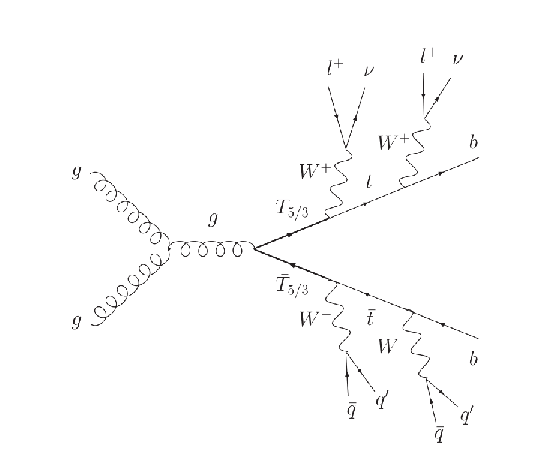
\includegraphics[width=\textwidth]{images/pdf/TTbar_feynman}
    \caption{Pair-production of the \TP, decaying into same-sign leptons and
    at least four jets.}
    \label{fig:TTbar_feynman}
\end{figure}

The backgrounds associated with this signal can be divided into three
categories:
\begin{description}\label{page:background_categories}
    \item[two same-sign prompt leptons] from rare SM processes.
    \item[opposite-sign leptons] whose charge is mismeasured, leading to a
        same-sign final state.
    \item[one prompt and one non-prompt lepton with the same charge] (or two
        non-prompt same-sign leptons). This background arises mainly from
        \ttbar events where one of the leptons comes from the decay of a
        $b$ quark, but is mistaken for a prompt lepton.
\end{description}

In order to reject all of these background sources, the following baseline
selection is applied:
\begin{itemize}
    \item event cleanup and trigger
    \item exactly two same-sign leptons, rejecting events with three or more
        leptons
    \item quarkonia veto, with the invariant mass of the leptons greater
        than \unit[20]{GeV}
    \item \Z veto, with the invariant mass of the \E\E and \M\M pairs not in
        the 76-106 window. This selection is not needed for \E\M
        events for lepton number conservation.
    \item at least four jets
\end{itemize}
The event cleanup and trigger requirements are detailed
in~\ref{sec:event_cleanup} and~\ref{sec:triggers}.
The invariant mass selections are particularly well suited to 
reject events with charge misidentification, in addition to the charge
consistency requirement on page~\pageref{page:electron_charge}, particularly from $\Z
\rightarrow \E\E$ decays or production of light mesons. 
The distribution of the number of jets in the signal and backgrounds
(figure~\ref{fig:n_jets}) also
shows that this is a good discriminating variable against both the
prompt and the \ttbar backgrounds.

\begin{figure}[htb]
    \centering
    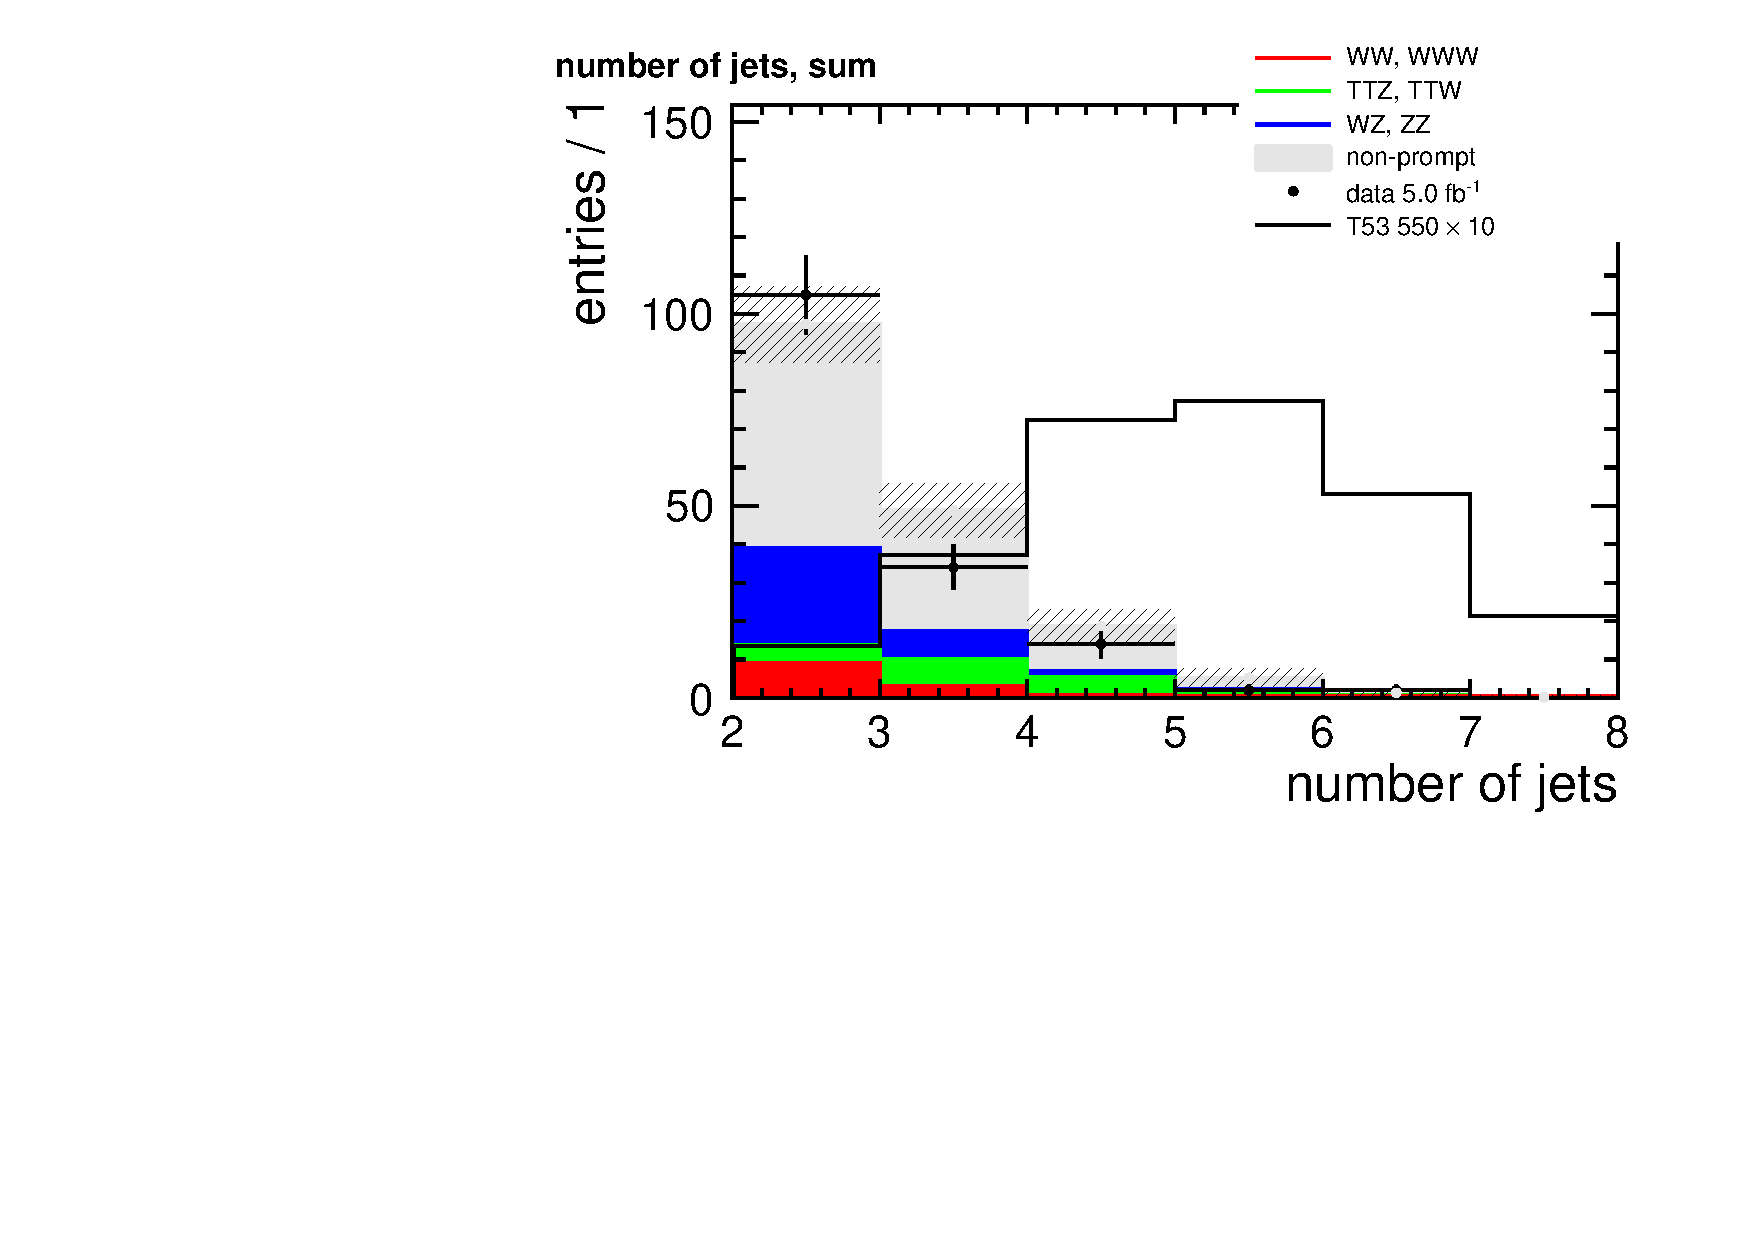
\includegraphics[width=\textwidth]{images/pdf/n_jets_sum}

    \caption{Distribution of the number of jets in the backgrounds and
        signal for the \unit[550]{GeV} mass point for the sum of the three channels:
    \E\E, \E\M\ and \M\M. The signal is amplified by factor of ten.}
    \label{fig:n_jets}
\end{figure}

While the prompt same-sign background is modelled by the Monte Carlo, we
found that a data-driven method is needed for an accurate description of the
contributions from charge misidentification and non-prompt leptons.
That is the subject of the following chapter.

% ********************************************************************
% Backmatter
%*******************************************************
%\appendix
%\cleardoublepage
%\part{Appendix}
%\include{chapters/Chapter0A}
%********************************************************************
% Other Stuff in the Back
%*******************************************************
\cleardoublepage%********************************************************************
% Bibliography
%*******************************************************
% work-around to have small caps also here in the headline
\manualmark
\markboth{\spacedlowsmallcaps{\bibname}}{\spacedlowsmallcaps{\bibname}} % work-around to have small caps also
%\phantomsection 
\refstepcounter{dummy}
\addtocontents{toc}{\protect\vspace{\beforebibskip}} % to have the bib a bit from the rest in the toc
\addcontentsline{toc}{chapter}{\tocEntry{\bibname}}
\bibliographystyle{plainnat}
\label{app:bibliography} 
\bibliography{bibliography}

% ********************************************************************
% Game Over: Restore, Restart, or Quit?
%*******************************************************
\end{document}
